\documentclass[a4paper,12pt, titlepage]{report}
\usepackage{polski}
\usepackage[polish]{babel}
\usepackage[utf8]{inputenc} % set input encoding (not needed with XeLaTeX
\usepackage{placeins}
\usepackage{graphicx} % support the \includegraphics command and options

% \usepackage[parfill]{parskip} % Activate to begin paragraphs with an empty line rather than an indent

%%% PACKAGES
\usepackage{booktabs} % for much better looking tables
\usepackage{array} % for better arrays (eg matrices) in maths
\usepackage{paralist} % very flexible & customisable lists (eg. enumerate/itemize, etc.)
\usepackage{verbatim} % adds environment for commenting out blocks of text & for better verbatim
\usepackage{subfig} % make it possible to include more than one captioned figure/table in a single float

\usepackage[a4paper,width=150mm,top=25mm,bottom=25mm]{geometry}
\usepackage{lmodern}  % for bold teletype font
\usepackage{amsmath}  % for \hookrightarrow
\usepackage{xcolor}   % for \textcolor
\usepackage{listings}
\lstset{
  basicstyle=\ttfamily,
  columns=fullflexible,
  frame=single,
  breaklines=true,
  postbreak=\mbox{\textcolor{red}{$\hookrightarrow$}\space},
}
%%% HEADERS & FOOTERS
\usepackage{fancyhdr} % This should be set AFTER setting up the page geometry
\pagestyle{fancy} % options: empty , plain , fancy
\renewcommand{\headrulewidth}{0pt} % customise the layout...
\lhead{}\chead{}\rhead{}
\lfoot{}\cfoot{\thepage}\rfoot{}
\fancyfoot{}

%%% SECTION TITLE APPEARANCE
\usepackage{sectsty}
\allsectionsfont{\sffamily\mdseries\upshape} % (See the fntguide.pdf for font help)
% (This matches ConTeXt defaults)

%%% ToC (table of contents) APPEARANCE
\usepackage[nottoc,notlof,notlot]{tocbibind} % Put the bibliography in the ToC
\usepackage[titles,subfigure]{tocloft} % Alter the style of the Table of Contents
\renewcommand{\cftsecfont}{\rmfamily\mdseries\upshape}
\renewcommand{\cftsecpagefont}{\rmfamily\mdseries\upshape} % No bold!

\graphicspath{ {./images/} }

\def\uczelnia{{Uniwersytet Kardynała Stefana Wyszyńskiego w~Warszawie}\\
Wydział Matematyczno-Przyrodniczy \\ Szkoła Nauk Ścisłych}
\def\nralbumu{107418}
\title{Przetwarzanie obrazów\\Sprawozdanie z laboratorium}
\author{Małgorzata Wiśniewska}
\date{Warszawa, 2020} 

\begin{document}
\maketitle
\tableofcontents
\chapter{Wstęp}
\section{Format obrazów}
\section{Instrukcja obsługi programu}

\chapter{Operacje ujednolicania obrazów}
Operacje ujednolicania obrazów dzieli się na dwa etapy. Pierwszym etapem jest ujednolicanie geometryczne, drugim jest ujednolicenie rozdzielczościowe. W prezentowanym programie ujednolicane są dwa obrazy, w taki sposób, że mniejszy z nich jest doprowadzany do takiego samego rozmiaru jak większy. Skutkuje to wygenerowaniem nowego obrazu o zwiększonej ilości piksli niż początkowa wartość. Dzięki zastosowaniu tego typu ujednolicania w efekcie nie następuje widoczny spadek jakości. 
\section{Ujednolicanie obrazów szarych geometryczne}
\subsection*{Opis algorytmu}
\par Operacje geometrycznego ujednolicania polega na wyrównaniu liczby piksli w kolumnach i wierszach w obu obrazach, poprzez zwiększenie liczby piksli w kolumnach i wierszach mniejszego z obrazów.
\begin{enumerate}
\item Wybierz największą wysokość i największą szerokość spośród obu obrazów.
\item Jeśli dany obraz ma mniejszą wysokość lub szerokość, wypełnij różnicę pikslami o wartości 1, tak, żeby wysokość i szerokość obu obrazów była równa.
\end{enumerate}
\subsection*{Efekty wykorzystania algorytmu}
\begin{figure}[h]
    \centering
    \subfloat[Obraz 1: 256x256]{{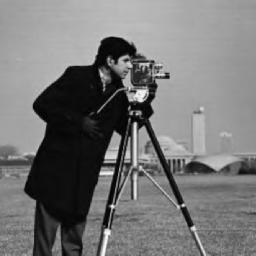
\includegraphics[width=0.4\textwidth]{./RawPictures/fotograf.png} }}%
    \qquad
    \subfloat[Obraz 2: 512x512]{{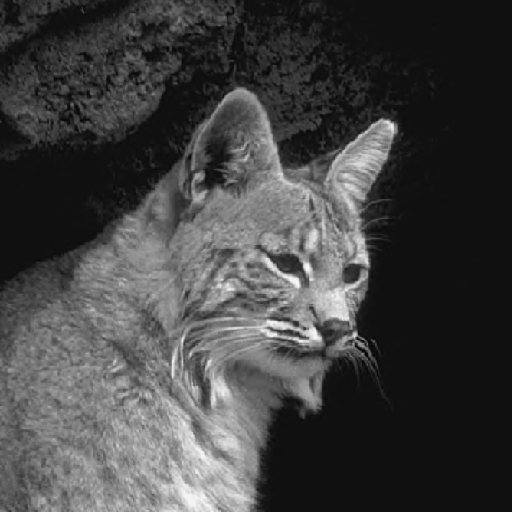
\includegraphics[width=0.4\textwidth]{./RawPictures/rys.png} }}%
    \caption{Obrazy wejściowe}%
    \label{fig:geo_before_grey1}%
\end{figure}
\FloatBarrier
\begin{figure}[h]
    \centering
    \subfloat[Obraz 1: 512x512]{{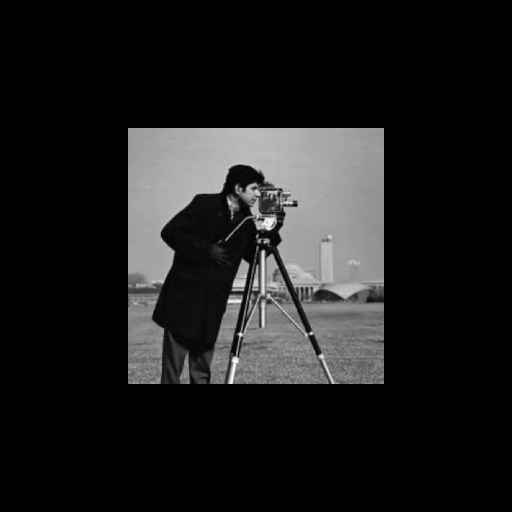
\includegraphics[width=0.4\textwidth]{./ExEffects/1/11/fotograf_rys.png} }}%
    \qquad
    \subfloat[Obraz 2: 512x512]{{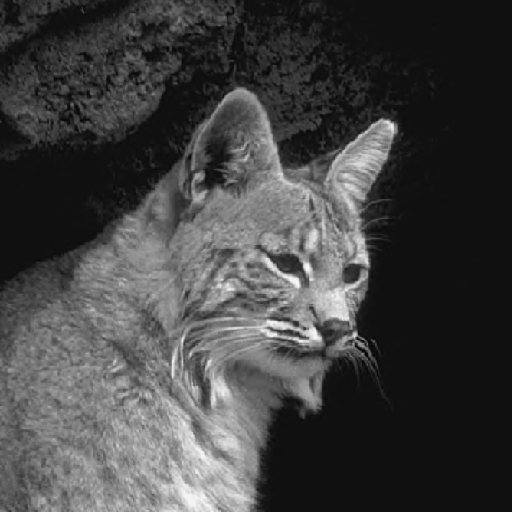
\includegraphics[width=0.4\textwidth]{./RawPictures/rys.png} }}%
    \caption{Obrazy wyjściowe}%
    \label{fig:geo_after_grey1}%
\end{figure}
\FloatBarrier
\begin{figure}[h]
    \centering
    \subfloat[Obraz 1: 369x480]{{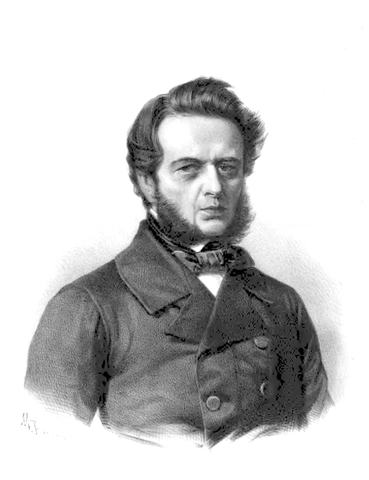
\includegraphics[width=0.4\textwidth]{./RawPictures/AndrzejZamoyski.png} }}%
    \qquad
    \subfloat[Obraz 2: 623x640]{{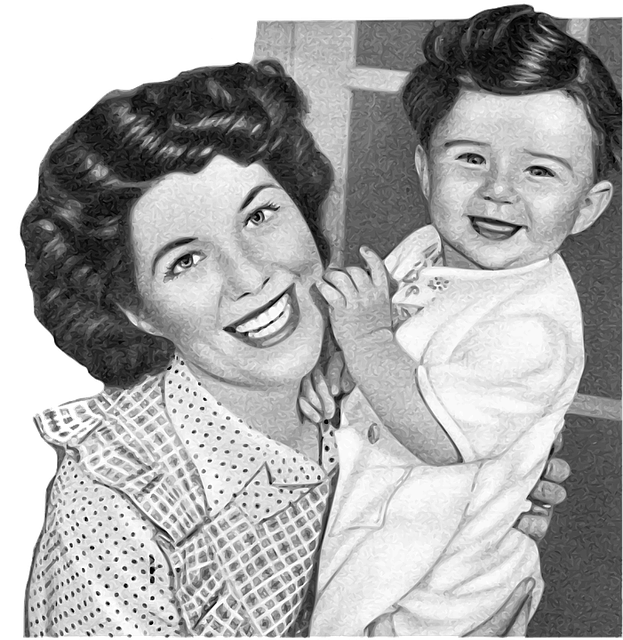
\includegraphics[width=0.4\textwidth]{./RawPictures/kobietaDziecko.png} }}%
    \caption{Obrazy wejściowe}%
    \label{fig:geo_before_grey2}%
\end{figure}
\FloatBarrier
\begin{figure}[h]
    \centering
    \subfloat[Obraz 1:  623x640]{{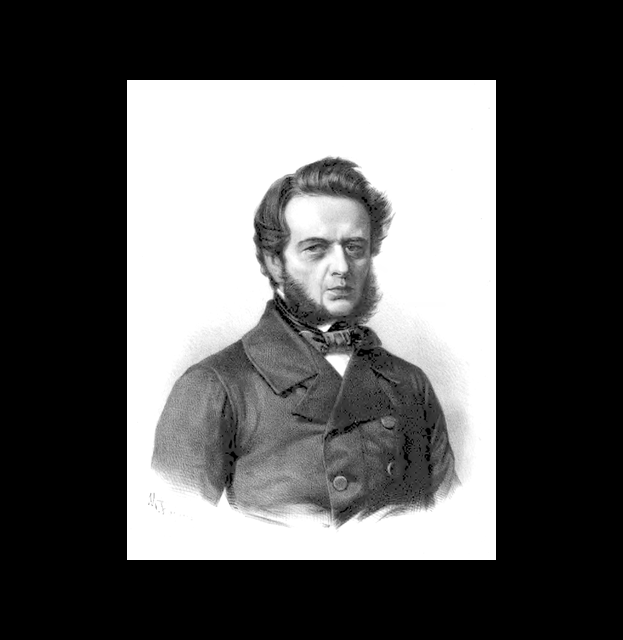
\includegraphics[width=0.4\textwidth]{./ExEffects/1/11/AndrzejZamoyski_kobietaDziecko.png} }}%
    \qquad
    \subfloat[Obraz 2:  623x640]{{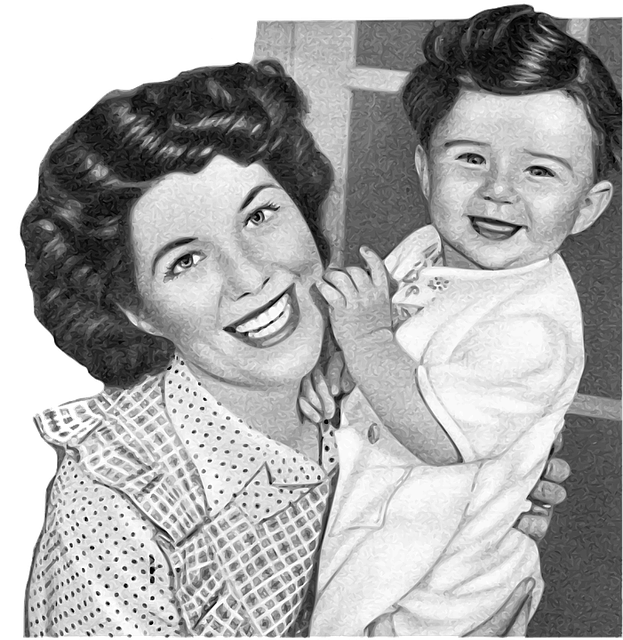
\includegraphics[width=0.4\textwidth]{./RawPictures/kobietaDziecko.png} }}%
    \caption{Obrazy wyjściowe}%
    \label{fig:geo_after_grey2}%
\end{figure}
\FloatBarrier
\subsection*{Kod źródłowy algorytmu}
\begin{lstlisting}[language=Python]
def geoUnificationGrey(self):
	# porownaj wielkosc obrazow, jezeli sa tego samego rozmiaru nie rob nic
	if self.biggerPicture == 0 and self.smallerPicture == 0:
		print('Both pictures have the same size')
		return 0
	# stworz tablice zer do zapisu efektu algorytmu
	result = np.zeros((self.maxLength, self.maxWidth), np.uint8)
	startWidthIndex = int(round((self.maxWidth - self.minWidth) / 2))
	startLengthIndex = int(round((self.maxLength - self.minLength) / 2))
	for w in range(0, self.minWidth):
		for l in range(0, self.minLength):
			result[l + startLengthIndex, w + startWidthIndex] = self.matrix[l, w]
	#zapisz zunifikowany obraz
	path = self.ex + self.smallerPictureName + '_' + self.biggerPictureName + '.png'
	self.saver.savePictureFromArray(result, 'L', path)
\end{lstlisting}

\section{Ujednolicanie obrazów szarych rozdzielczościowe}
\subsection*{Opis algorytmu}
\par Operacja rozdzielczościowego ujednolicania obrazów następuje po ujednoliceniu geometrycznym obrazów wejściowych. Polega na wypełnieniu obrazu pikslami. Brakujące piksle powinny zostać zinterpolowane.
\begin{enumerate}
\item Wypełnij cały obraz pikslami o znanej wartości zachowując pewien odstęp między nimi, gdzie odstępem będą piksle o wartości 0.
\item Każdemu pikslowi o nieznanej wartości przypisz średnią wartość znanych (>0) piksli z jego bezpośredniego otoczenia.
\end{enumerate}
\subsection*{Efekty wykorzystania algorytmu}
\begin{figure}[h]
    \centering
    \subfloat[Obraz 1: 512x512]{{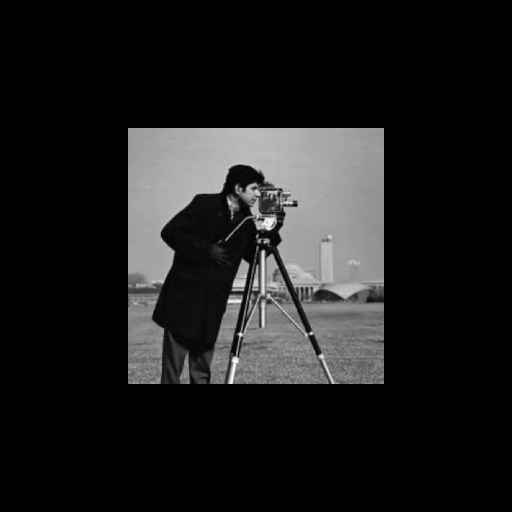
\includegraphics[width=0.4\textwidth]{./ExEffects/1/11/fotograf_rys.png} }}%
    \qquad
    \subfloat[Obraz 2: 512x512]{{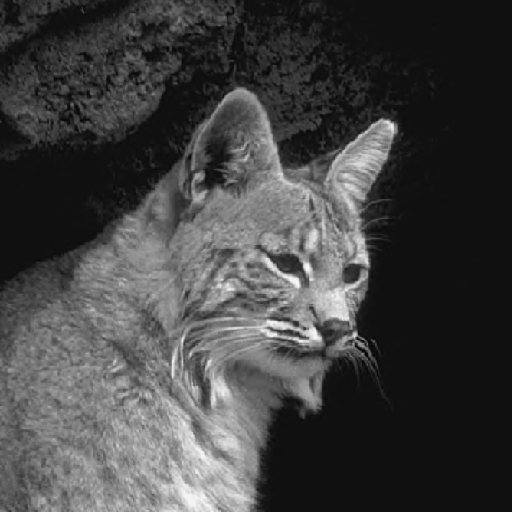
\includegraphics[width=0.4\textwidth]{./RawPictures/rys.png} }}%
    \caption{Obrazy wejściowe po ujednoliceniu geometrycznym}%
    \label{fig:example}%
\end{figure}
\FloatBarrier
\begin{figure}[h]
    \centering
    \subfloat[Obraz 1: 512x512]{{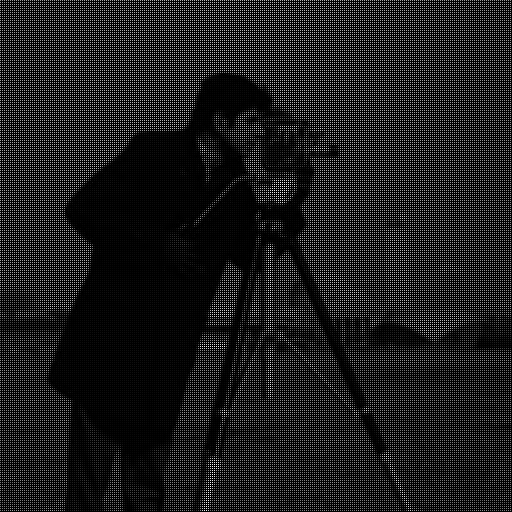
\includegraphics[width=0.4\textwidth]{./ExEffects/1/12/fotograf_rys_withoutInterpolation.png} }}%
    \qquad
    \subfloat[Obraz 2: 512x512]{{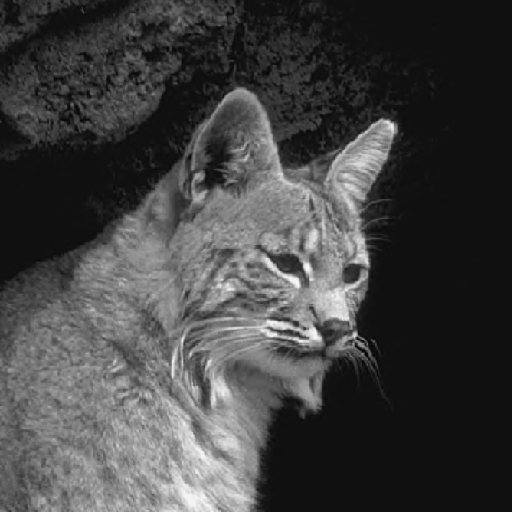
\includegraphics[width=0.4\textwidth]{./RawPictures/rys.png} }}%
    \caption{Obrazy wyjściowe bez interpolacji}%
    \label{fig:example}%
\end{figure}
\FloatBarrier
\begin{figure}[h]
    \centering
    \subfloat[Obraz 1: 512x512]{{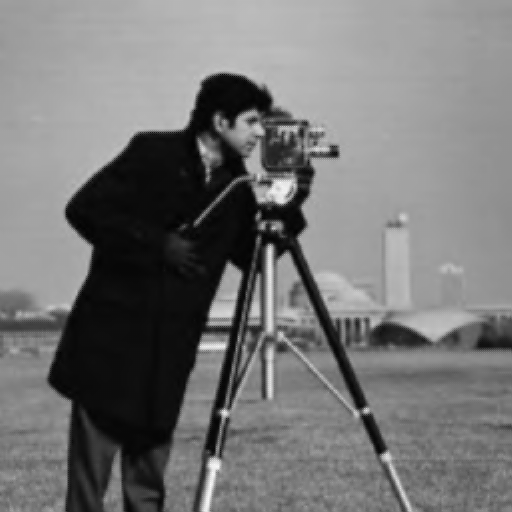
\includegraphics[width=0.4\textwidth]{./ExEffects/1/12/fotograf_rys_withInterpolation.png} }}%
    \qquad
    \subfloat[Obraz 2: 512x512]{{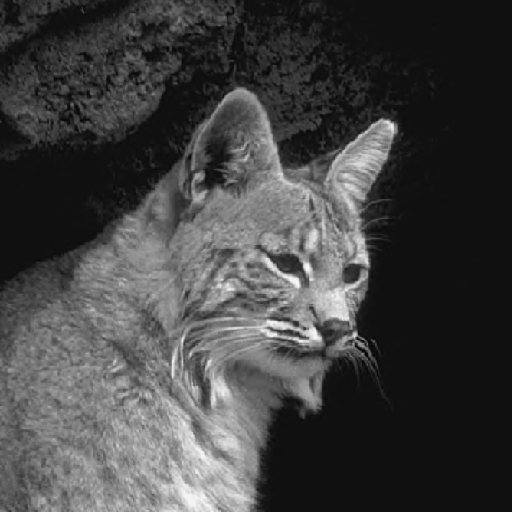
\includegraphics[width=0.4\textwidth]{./RawPictures/rys.png} }}%
    \caption{Obrazy wyjściowe po interpolacji}%
    \label{fig:example}%
\end{figure}
\FloatBarrier
\subsection*{Kod źródłowy algorytmu}
\begin{lstlisting}[language=Python]
def resolutionUnificationGrey(self):
    print('Beginning of resolution unification for two grey pictures.')
    if self.biggerPicture == 0 and self.smallerPicture == 0:
        print('Both pictures have the same size')
        return 0
    scaleFactorLength = float(self.maxLength / self.minLength)
    scaleFactorWidth = float(self.maxWidth / self.minWidth)
    result = np.zeros((self.maxLength, self.maxWidth), np.uint8)
    for l in range(self.minLength):
        for w in range(self.minWidth):
            if w % 2 == 0:
                pomL = int(scaleFactorLength * l)
                pomW = int(round(scaleFactorWidth * w))
                result[pomL, pomW] = self.matrix[l, w]
            elif w % 2 == 1:
                pomL = int(round(scaleFactorLength * l))
                pomW = int(scaleFactorWidth * w)
                result[pomL, pomW] = self.matrix[l, w]
    # zapisz obraz bez interpolacji
    path = self.ex + self.smallerPictureName + '_' + self.biggerPictureName + '_withoutInterpolation.png'
    self.saver.savePictureFromArray(result, 'L', path)
    # interpolacja
    for l in range(self.maxLength):
        for w in range(self.maxWidth):
            value = 0
            count = 0
            if result[l, w] == 0:
                for lOff in range(-1, 2):
                    for wOff in range(-1, 2):
                        lSave = l if ((l + lOff) > (self.maxLength - 2)) | ((l + lOff) < 0) else (l + lOff)
                        wSave = w if ((w + wOff) > (self.maxWidth - 2)) | ((w + wOff) < 0) else (w + wOff)
                        if result[lSave, wSave] != 0:
                            value += result[lSave, wSave]
                            count += 1
                result[l, w] = value / count
    # zapisz obraz po interpolacji
    path = self.ex + self.smallerPictureName + '_' + self.biggerPictureName + '_withInterpolation.png'
    self.saver.savePictureFromArray(result, 'L', path)
    print('Finished resolution unification.')
\end{lstlisting}

\section{Ujednolicanie obrazów RGB geometryczne}
\subsection*{Opis algorytmu}
\par Operacje geometrycznego ujednolicania polega na wyrównaniu liczby piksli w kolumnach i wierszach w obu obrazach, poprzez zwiększenie liczby piksli w kolumnach i wierszach mniejszego z obrazów.
\begin{enumerate}
\item Wybierz największą wysokość i największą szerokość spośród obu obrazów.
\item Jeśli dany obraz ma mniejszą wysokość lub szerokość, wypełnij różnicę pikslami o wartości 1 dla każdego z kanałów (R,G,B), tak, żeby wysokość i szerokość obu obrazów była równa.
\end{enumerate}
\subsection*{Efekty wykorzystania algorytmu}
\begin{figure}[h]
    \centering
    \subfloat[Obraz 1: 512x512]{{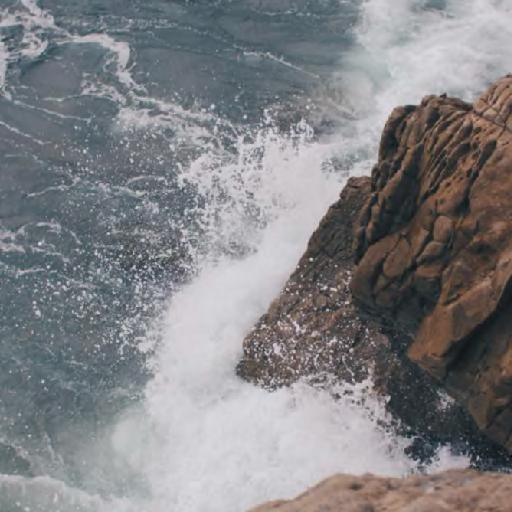
\includegraphics[width=0.4\textwidth]{./RawPictures/morze.png} }}%
    \qquad
    \subfloat[Obraz 2: 1025x1025]{{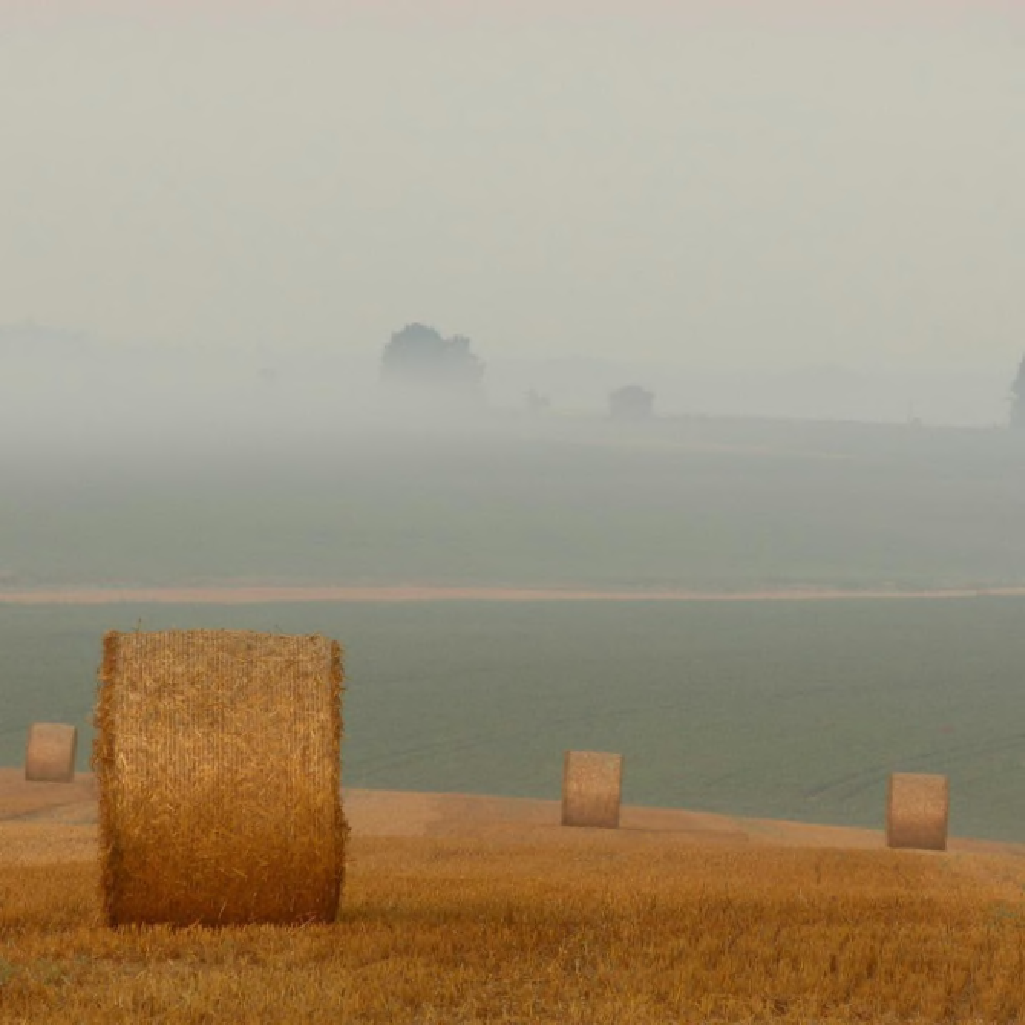
\includegraphics[width=0.4\textwidth]{./RawPictures/stogi.png} }}%
    \caption{Obrazy wejściowe}%
    \label{fig:geo_before_grey1}%
\end{figure}
\FloatBarrier
\begin{figure}[h]
    \centering
    \subfloat[Obraz 1: 1025x1025]{{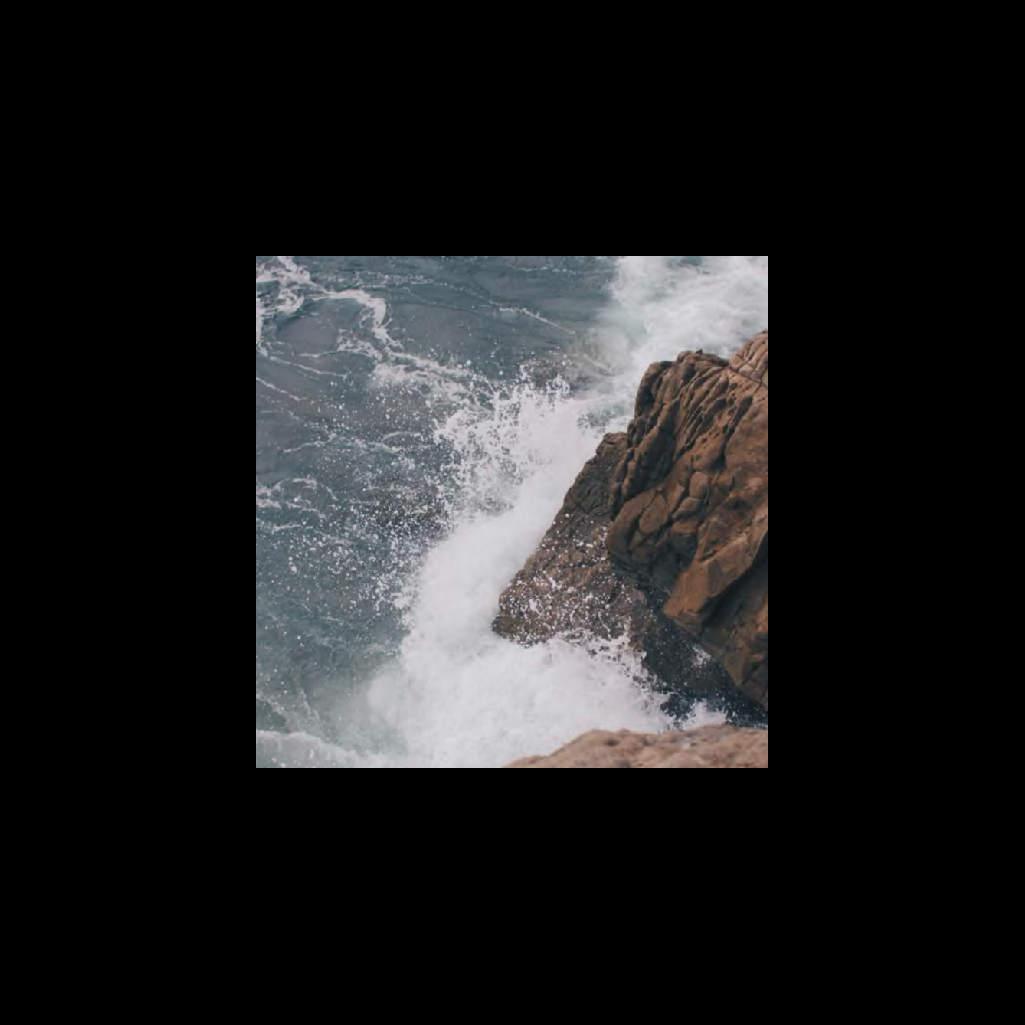
\includegraphics[width=0.4\textwidth]{./ExEffects/1/13/morze_stogi.png} }}%
    \qquad
    \subfloat[Obraz 2: 1025x1025]{{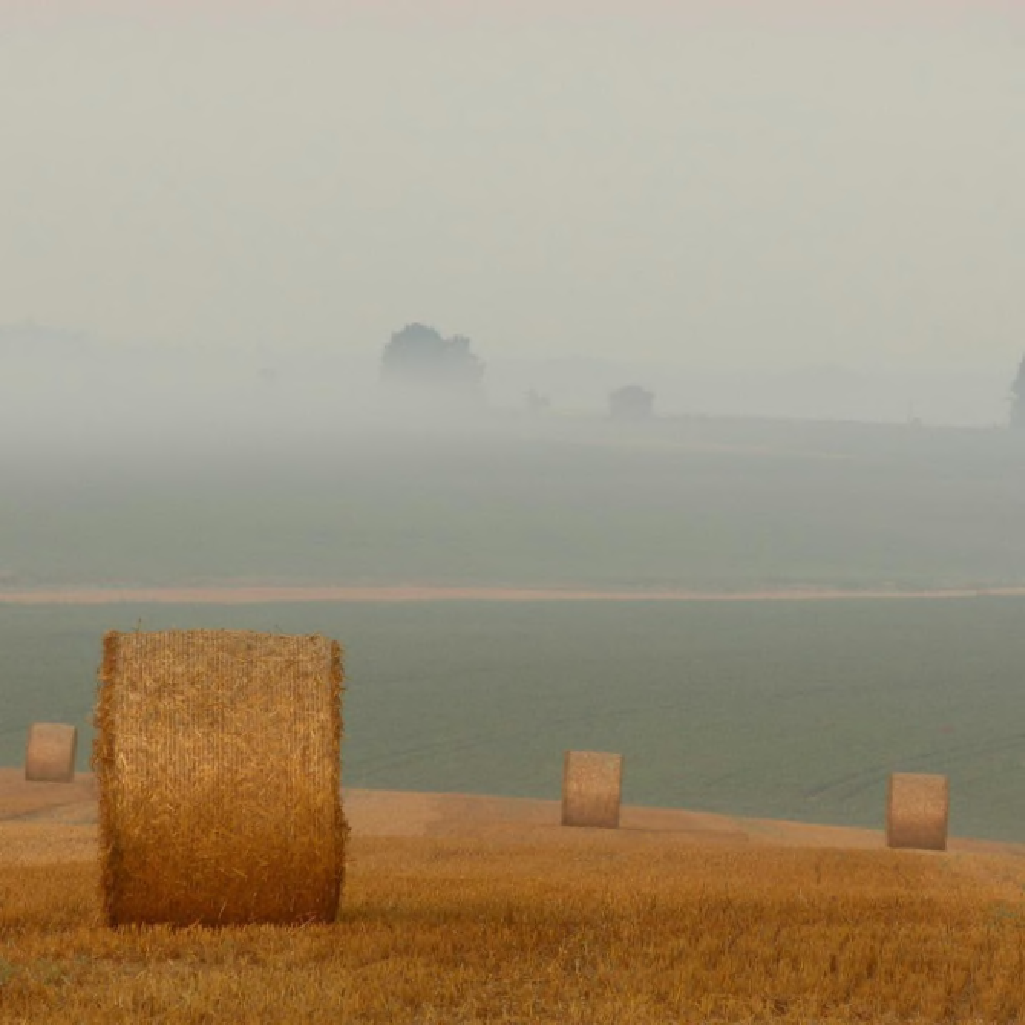
\includegraphics[width=0.4\textwidth]{./RawPictures/stogi.png} }}%
    \caption{Obrazy wyjściowe}%
    \label{fig:geo_after_grey1}%
\end{figure}
\FloatBarrier
\begin{figure}[h]
    \centering
    \subfloat[Obraz 1: 256x256]{{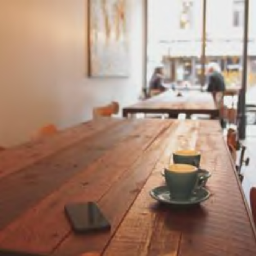
\includegraphics[width=0.4\textwidth]{./RawPictures/kawa.png} }}%
    \qquad
    \subfloat[Obraz 2: 512x512]{{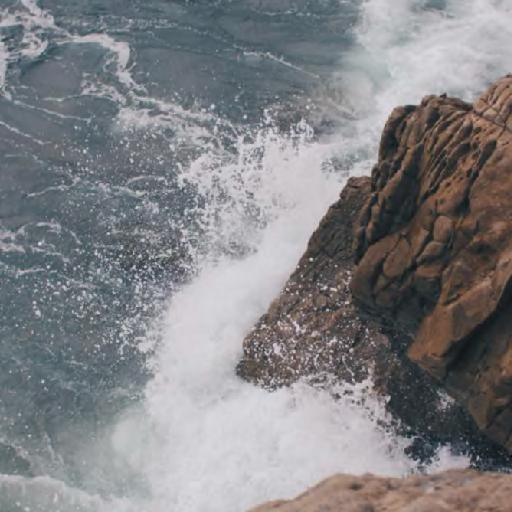
\includegraphics[width=0.4\textwidth]{./RawPictures/morze.png} }}%
    \caption{Obrazy wejściowe}%
    \label{fig:geo_before_grey2}%
\end{figure}
\FloatBarrier
\begin{figure}[h]
    \centering
    \subfloat[Obraz 1:  512x512]{{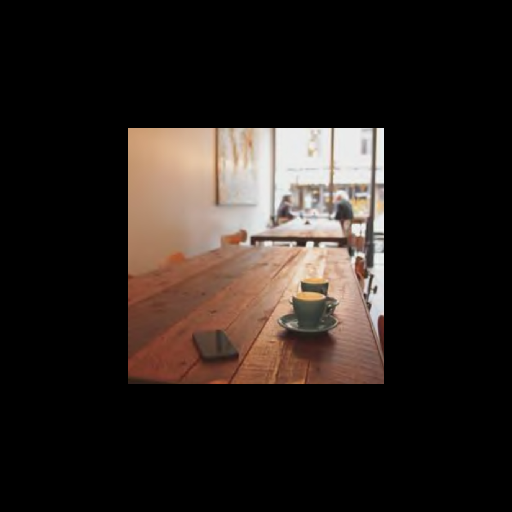
\includegraphics[width=0.4\textwidth]{./ExEffects/1/13/kawa_morze.png} }}%
    \qquad
    \subfloat[Obraz 2:  512x512]{{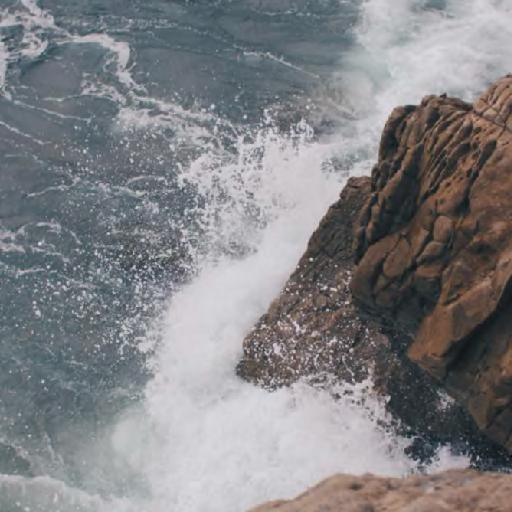
\includegraphics[width=0.4\textwidth]{./RawPictures/morze.png} }}%
    \caption{Obrazy wyjściowe}%
    \label{fig:geo_after_grey2}%
\end{figure}
\FloatBarrier
\subsection*{Kod źródłowy algorytmu}
\begin{lstlisting}[language=Python]
def geoUnificationRGB(self):
    if self.biggerPicture == 0 and self.smallerPicture == 0:
        print('Both pictures have the same size')
        return 0
    # stworz tablice z zerami jako odstawe dla unifikacji
    result = np.full((self.maxLength, self.maxWidth, 3), 0, np.uint8)
    startWidthIndex = int(round((self.maxWidth - self.minWidth) / 2))
    startLengthIndex = int(round((self.maxLength - self.minLength) / 2))
    for w in range(0, self.minWidth):
        for l in range(0, self.minLength):
            result[l + startLengthIndex, w + startWidthIndex] = self.matrix[w, l]
    # zapisz zunifikowany obraz
    path = self.ex + self.smallerPictureName + '_' + self.biggerPictureName + '.png'
    self.saver.savePictureFromArray(result, 'RGB', path)
\end{lstlisting}

\section{Ujednolicanie obrazów RGB rozdzielczościowe}
\subsection*{Opis algorytmu}
\par Operacja rozdzielczościowego ujednolicania obrazów następuje po ujednoliceniu geometrycznym obrazów wejściowych. Polega na wypełnieniu obrazu pikslami. Brakujące piksle powinny zostać zinterpolowane.
\begin{enumerate}
\item Wypełnij cały obraz pikslami o znanej wartości zachowując pewien odstęp między nimi, gdzie odstępem będą piksle o wartości 0.
\item Każdemu pikslowi (ze wszystkich kanałów - R, G, B) o nieznanej wartości przypisz średnią wartość znanych (>0) piksli z jego bezpośredniego otoczenia.
\end{enumerate}
\subsection*{Efekty wykorzystania algorytmu}
\begin{figure}[h]
    \centering
    \subfloat[Obraz 1: 1025x1025]{{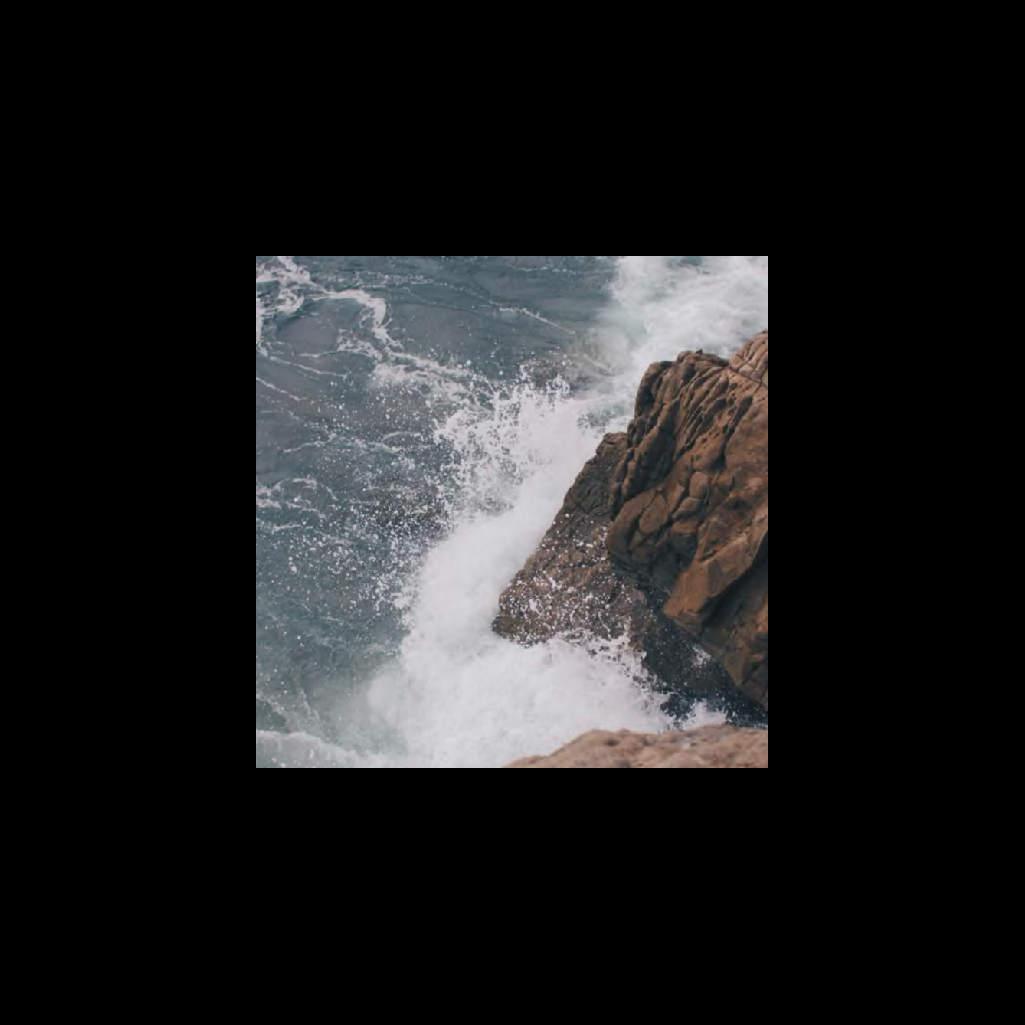
\includegraphics[width=0.4\textwidth]{./ExEffects/1/13/morze_stogi.png} }}%
    \qquad
    \subfloat[Obraz 2: 1025x1025]{{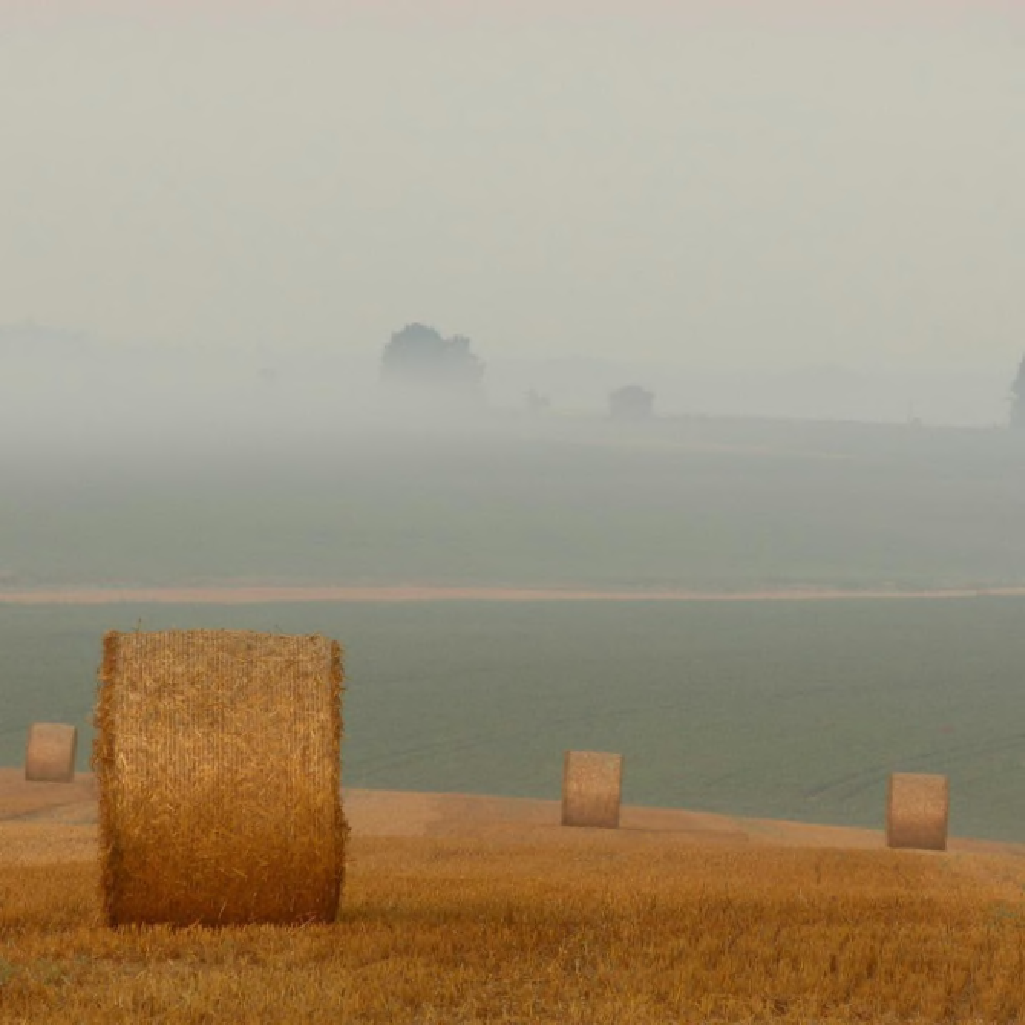
\includegraphics[width=0.4\textwidth]{./RawPictures/stogi.png} }}%
    \caption{Obrazy wejściowe po ujednoliceniu geometrycznym}%
    \label{fig:geo_after_grey1}%
\end{figure}
\FloatBarrier
\begin{figure}[h]
    \centering
    \subfloat[Obraz 1: 1025x1025]{{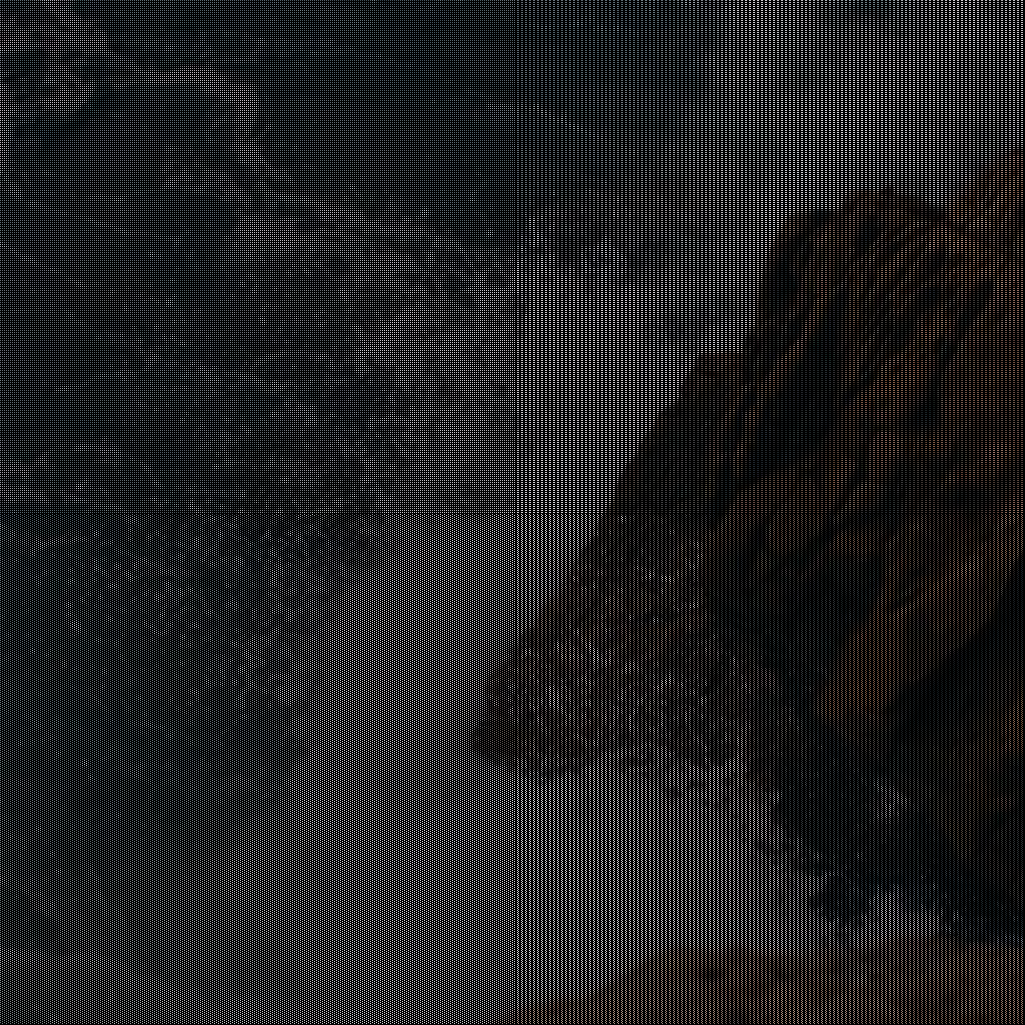
\includegraphics[width=0.4\textwidth]{./ExEffects/1/14/morze_stogi_withoutInterpolation.png} }}%
    \qquad
    \subfloat[Obraz 2: 1025x1025]{{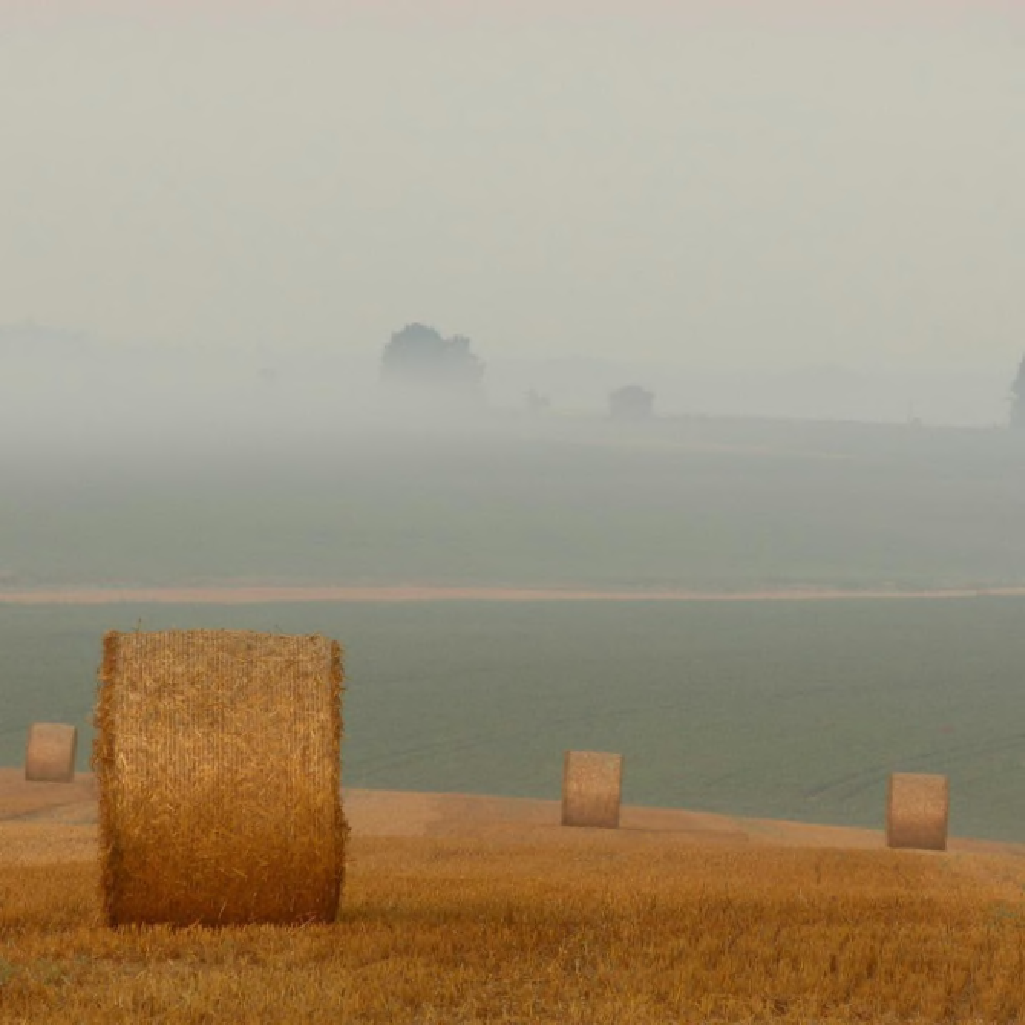
\includegraphics[width=0.4\textwidth]{./RawPictures/stogi.png} }}%
    \caption{Obrazy wyjściowe bez interpolacji}%
    \label{fig:example}%
\end{figure}
\FloatBarrier
\begin{figure}[h]
    \centering
    \subfloat[Obraz 1: 1025x1025]{{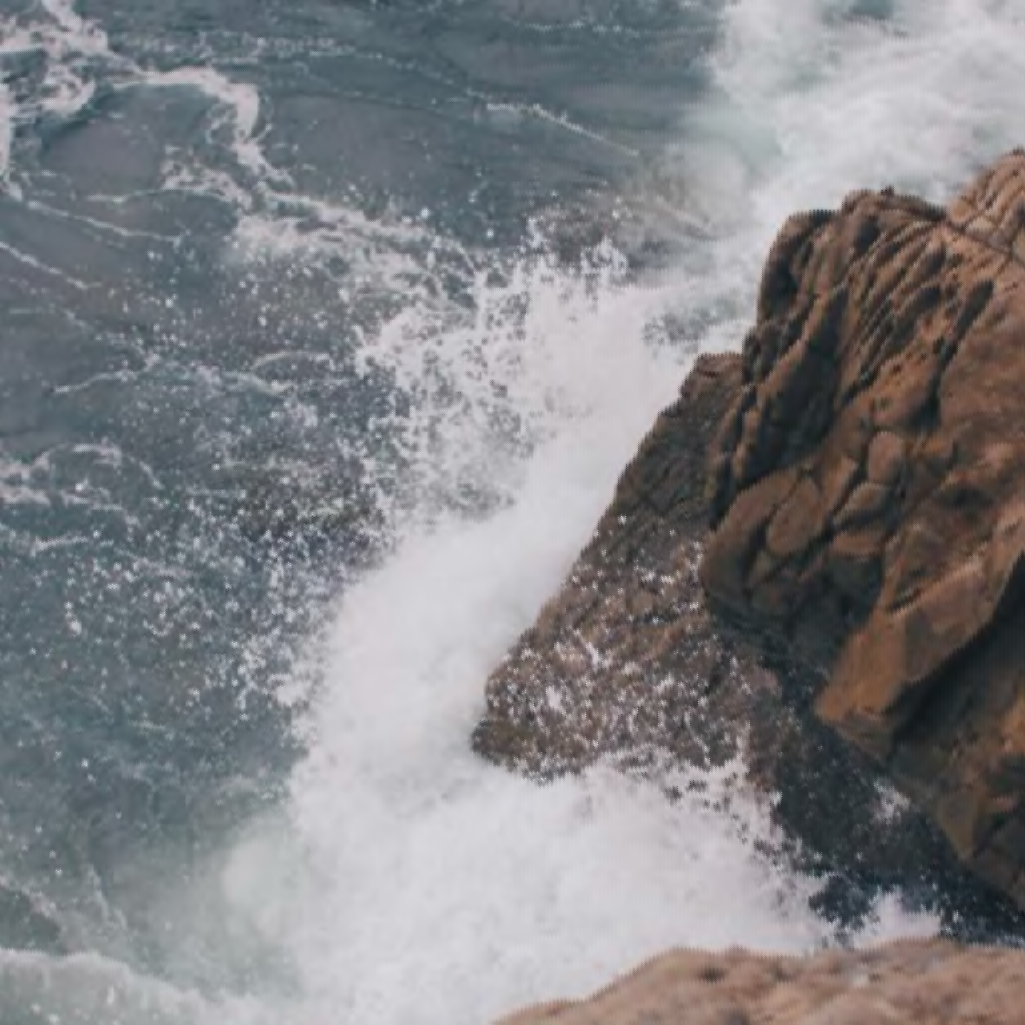
\includegraphics[width=0.4\textwidth]{./ExEffects/1/14/morze_stogi_withInterpolation.png} }}%
    \qquad
    \subfloat[Obraz 2: 1025x1025]{{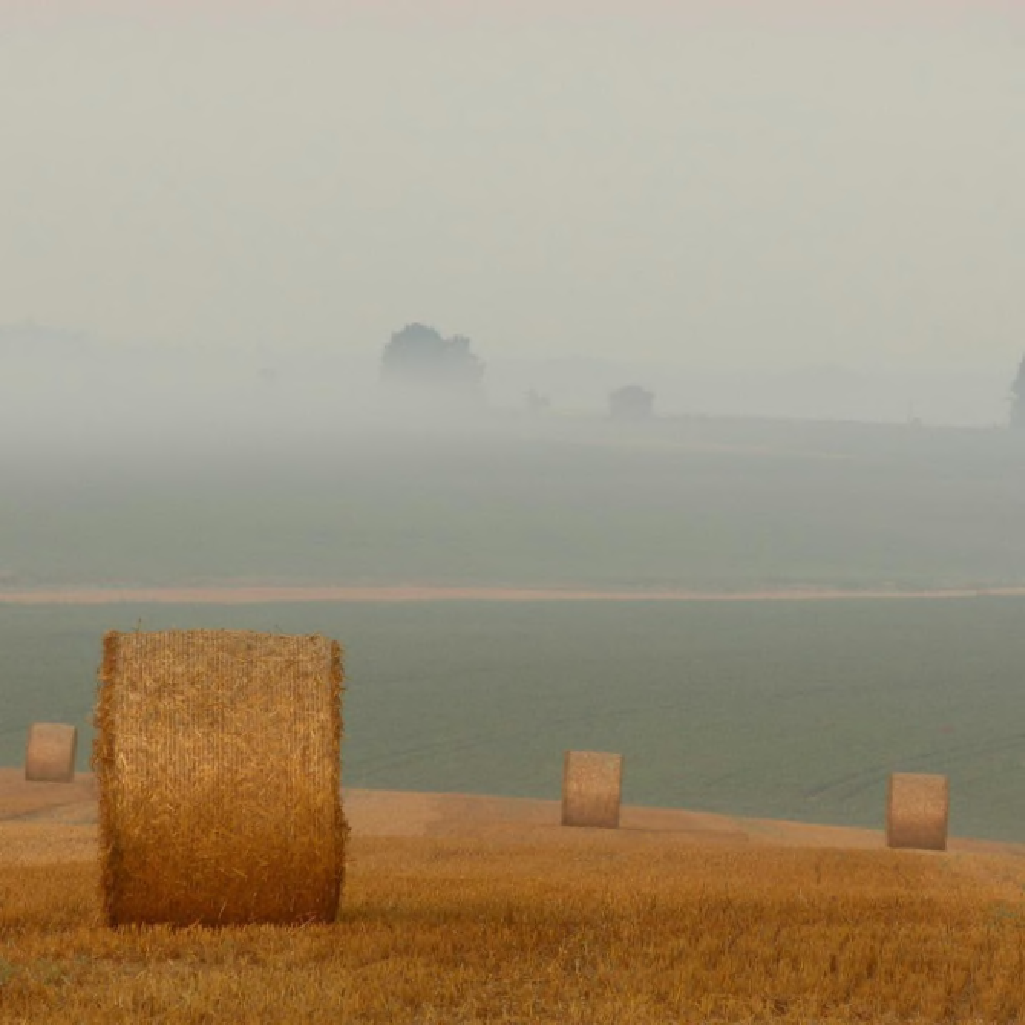
\includegraphics[width=0.4\textwidth]{./RawPictures/stogi.png} }}%
    \caption{Obrazy wyjściowe po interpolacji}%
    \label{fig:example}%
\end{figure}
\FloatBarrier
\subsection*{Kod źródłowy algorytmu}
\begin{lstlisting}[language=Python]
def resolutionUnificationGrey(self):
    print('Beginning of resolution unification for two grey pictures.')
    if self.biggerPicture == 0 and self.smallerPicture == 0:
        print('Both pictures have the same size')
        return 0
    scaleFactorLength = float(self.maxLength / self.minLength)
    scaleFactorWidth = float(self.maxWidth / self.minWidth)
    result = np.zeros((self.maxLength, self.maxWidth), np.uint8)
    for l in range(self.minLength):
        for w in range(self.minWidth):
            if w % 2 == 0:
                pomL = int(scaleFactorLength * l)
                pomW = int(round(scaleFactorWidth * w))
                result[pomL, pomW] = self.matrix[l, w]
            elif w % 2 == 1:
                pomL = int(round(scaleFactorLength * l))
                pomW = int(scaleFactorWidth * w)
                result[pomL, pomW] = self.matrix[l, w]
    # zapisz obraz bez interpolacji
    path = self.ex + self.smallerPictureName + '_' + self.biggerPictureName + '_withoutInterpolation.png'
    self.saver.savePictureFromArray(result, 'L', path)
    # interpolacja
    for l in range(self.maxLength):
        for w in range(self.maxWidth):
            value = 0
            count = 0
            if result[l, w] == 0:
                for lOff in range(-1, 2):
                    for wOff in range(-1, 2):
                        lSave = l if ((l + lOff) > (self.maxLength - 2)) | ((l + lOff) < 0) else (l + lOff)
                        wSave = w if ((w + wOff) > (self.maxWidth - 2)) | ((w + wOff) < 0) else (w + wOff)
                        if result[lSave, wSave] != 0:
                            value += result[lSave, wSave]
                            count += 1
                result[l, w] = value / count
    # zapisz obraz po interpolacji
    path = self.ex + self.smallerPictureName + '_' + self.biggerPictureName + '_withInterpolation.png'
    self.saver.savePictureFromArray(result, 'L', path)
    print('Finished resolution unification.')
\end{lstlisting}

\chapter{Operacje sumowania arytmetycznego obrazów szarych}
Operacje arytmtyczne między pikslami dwóch obrazów sa wykorzystywane w wielu działach przetwarzania obrazów. Przeprowadza się je wykonując operacje na pojedynczych pikslach. Po operacjach arytmetycznych zwykle konieczne jest normalizowanie obrazu wynikowego. W zadaniach do normalizacji wykorzystano wzór:
\[f{norm}=Z{rep}[(f-f{min})/(f{max}-f{min})]\]

\section{Sumowanie obrazów szarych z określoną stałą}
\subsection*{Opis algorytmu}
\par Algorytm sumowowania obrazu szarego z określoną stałą polega na daodaniu do każdej wartości pojedynczego piksla określonej stałej. Po operacji sumowania następuje normalizacja obrazu.
\begin{enumerate}
\item Policz sumy wartości każdego piksla ze stałą. Jeżeli suma przekracza 255 to konieczne jest
\begin{itemize}
\item Wybranie największej sumę piksla ze stałą - \(Q{max}\) 
\item Obliczenie \(D{max}\) ze wzoru: \(D{max}[l,w]=(Q{max}[l,w]-255)\)
\item Obliczenie \(X=D{max}/255\)
\end{itemize}
\item Policz sumę ze wzoru: \(Q[l,w]=P[l,w]-(P[l, w]*X)+const-(const*X)\)
\end{enumerate}
\subsection*{Efekty wykorzystania algorytmu}
\begin{figure}[h]
    \centering
    \subfloat{{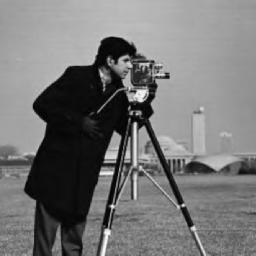
\includegraphics[width=0.3\textwidth]{./RawPictures/fotograf.png} }}%
    \subfloat{{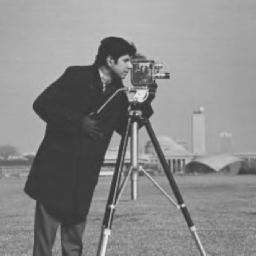
\includegraphics[width=0.3\textwidth]{./ExEffects/2/21/fotograf_constant_70.png} }}%
    \subfloat{{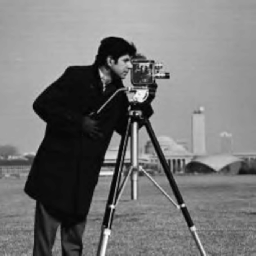
\includegraphics[width=0.3\textwidth]{./ExEffects/2/21/fotograf_constant_70_normalized.png} }}%
    \caption{[Od lewej] Szary obraz wejściowy, obraz po sumowaniu ze stałą 70, obraz po normalizacji}%
    \label{fig:geo_after_grey1}%
\end{figure}
\FloatBarrier
\begin{figure}[h]
    \centering
    \subfloat{{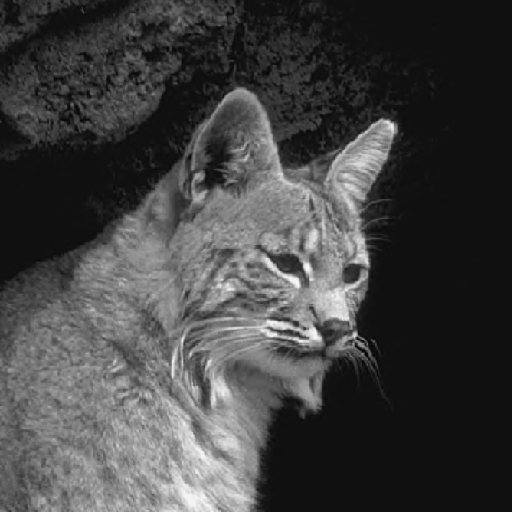
\includegraphics[width=0.3\textwidth]{./RawPictures/rys.png} }}%
    \subfloat{{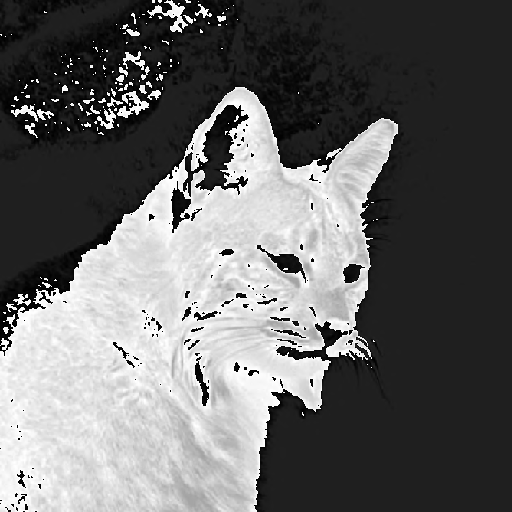
\includegraphics[width=0.3\textwidth]{./ExEffects/2/21/rys_constant_400.png} }}%
    \subfloat{{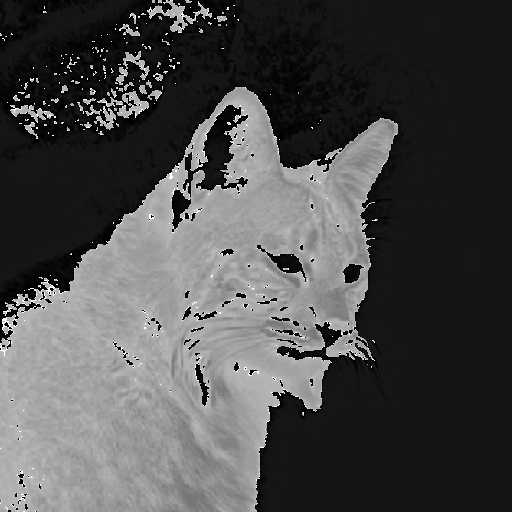
\includegraphics[width=0.3\textwidth]{./ExEffects/2/21/rys_constant_400_normalized.png} }}%
    \caption{[Od lewej] Szary obraz wejściowy, obraz po sumowaniu ze stałą 400, obraz po normalizacji}%
    \label{fig:geo_after_grey1}%
\end{figure}
\FloatBarrier
\subsection*{Kod źródłowy algorytmu}
\begin{lstlisting}[language=Python]
def addConstGrey(self, constant):
    maxBitsColor = self.checkPictureBits(self.pic1)
    length, width, pictureName = self.pic1.getPictureParameters()
    matrix = self.pic1.getGreyMatrix()
    result = np.ones((length, width), np.uint8)
    sumMax = 0
    x = 0
    fmin = maxBitsColor
    fmax = 0
    for l in range(length):
        for w in range(width):
            added = matrix[l, w] + constant
            if sumMax < added:
                sumMax = added
    if sumMax > maxBitsColor:
        x = (sumMax - maxBitsColor) / maxBitsColor
    for l in range(length):
        for w in range(width):
            # Rounded up and assignment of value to the result matrix
            pom = (matrix[l, w] - (matrix[l, w] * x)) + (constant - (constant * x))
            result[l, w] = np.ceil(pom)
            # Search for maximum and minimum
            if fmin > pom:
                fmin = pom
            if fmax < pom:
                fmax = pom
    # save picture with added constant to png file (without normalization)
    path = self.ex + str(pictureName) + '_constant_' + str(constant) + '.png'
    self.saver.savePictureFromArray(result, self.pictureType, path)
    for l in range(length):
        for w in range(width):
            result[l, w] = maxBitsColor*((result[l, w] - fmin) / (fmax - fmin))
    # save picture with added constant to png file (with normalization)
    path = self.ex + str(pictureName) + '_constant_' + str(constant) + '_normalized.png'
    self.saver.savePictureFromArray(result, self.pictureType, path)
\end{lstlisting}

\section{Sumowanie dwóch obrazów szarych}
\subsection*{Opis algorytmu}
\par Algorytm sumowowania obrazu szarego z drugim obrazem szarym jest określone tylko o tych samych wymiarach \(MxN\) i strukturze ich macierzy. Algorytm sumowania obrazu z obrazem polega na dodaniu do wartości piksla z  pierwszego obrazu, wartości odpowiadającego piksla z drugiego obrazu. Po operacji sumowania następuje normalizacja obrazu. Operacja dodawania obrazów są użyteczne przy uśrednianiu obrazów, w celu zredukowania na nich szumu.
\begin{enumerate}
\item Policz sumy wartości każdego piksla obrazu pierwszego \(P1[l,w]\) z odpowiadającym pikslem drugiego obrazu \(P2[l,w]\). Jeżeli suma przekracza 255 to konieczne jest
\begin{itemize}
\item Wybranie największej sumy odpowiadających piksli dwóch obrazów - \(Q{max}\) 
\item Obliczenie \(D{max}\) ze wzoru: \(D{max}[l,w]=(Q{max}[l,w]-255)\)
\item Obliczenie \(X=D{max}/255\)
\end{itemize}
\item Policz sumę ze wzoru: \(Q[l,w]=P1[l,w]-(P1[l,w]*X)+P2[l,w]-(P2[l,w]*X)\)
\end{enumerate}
\subsection*{Efekty wykorzystania algorytmu}
\begin{figure}[h]
    \centering
    \subfloat{{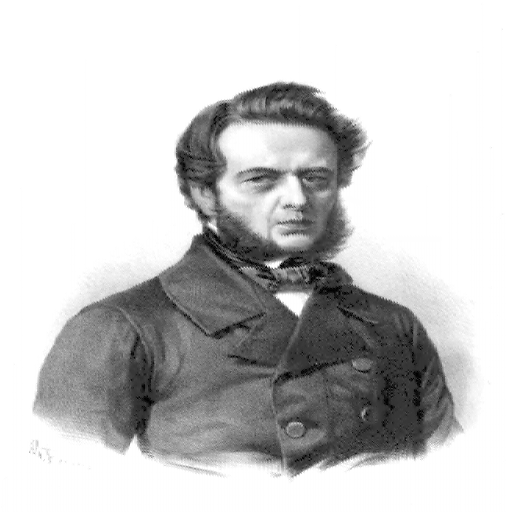
\includegraphics[width=0.4\textwidth]{./ExEffects/1/12/AndrzejZamoyski_rys_withInterpolation.png} }}%
    \subfloat{{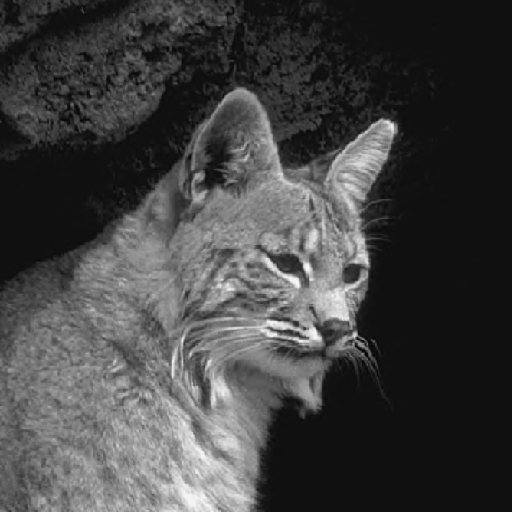
\includegraphics[width=0.4\textwidth]{./RawPictures/rys.png} }}%
    \qquad
    \subfloat{{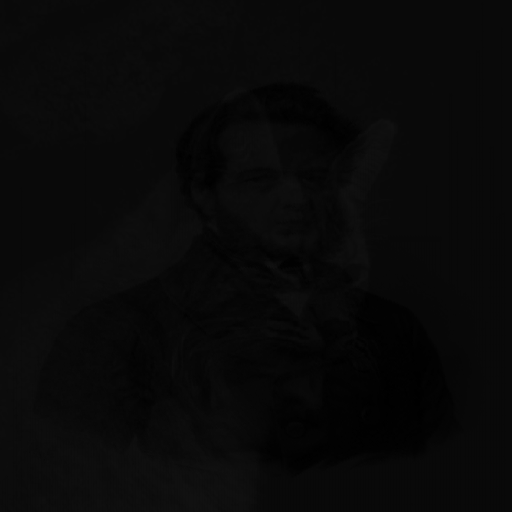
\includegraphics[width=0.4\textwidth]{./ExEffects/2/21/AndrzejZamoyski_added_rys.png} }}%
    \subfloat{{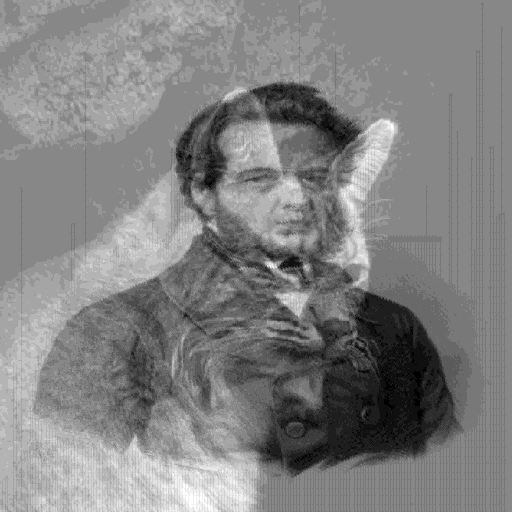
\includegraphics[width=0.4\textwidth]{./ExEffects/2/21/AndrzejZamoyski_added_rys_normalized.png} }}%
    \caption{[Od lewej, rząd 1] Szary obraz wejściowy 1, szary obraz wejściowy 2 [Od lewej, rząd 2] Obraz po sumowaniu obrazów 1 i 2, obraz po normalizacji}%
    \label{fig:geo_after_grey1}%
\end{figure}
\FloatBarrier
\begin{figure}[h]
    \centering
    \subfloat{{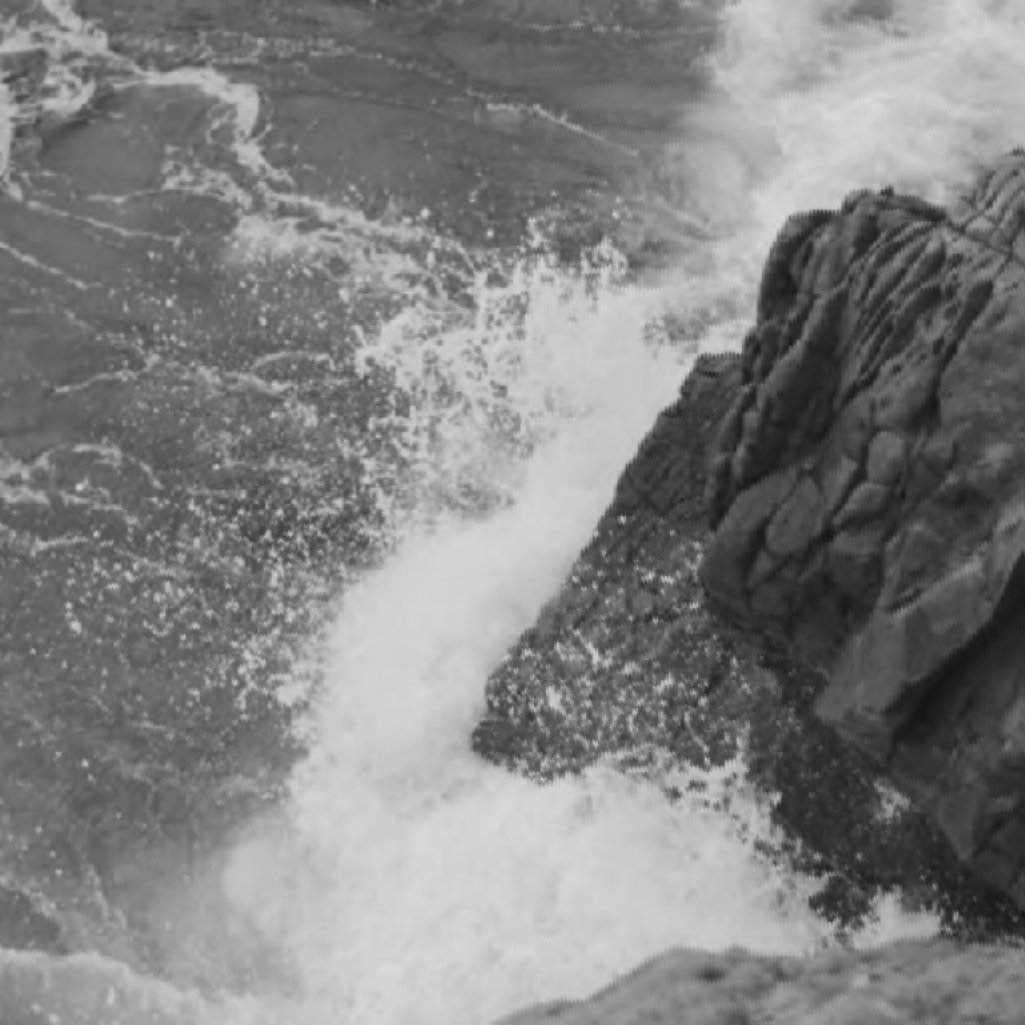
\includegraphics[width=0.4\textwidth]{./ExEffects/1/12/morze-szare_stogi-szare_withInterpolation.png} }}%
    \subfloat{{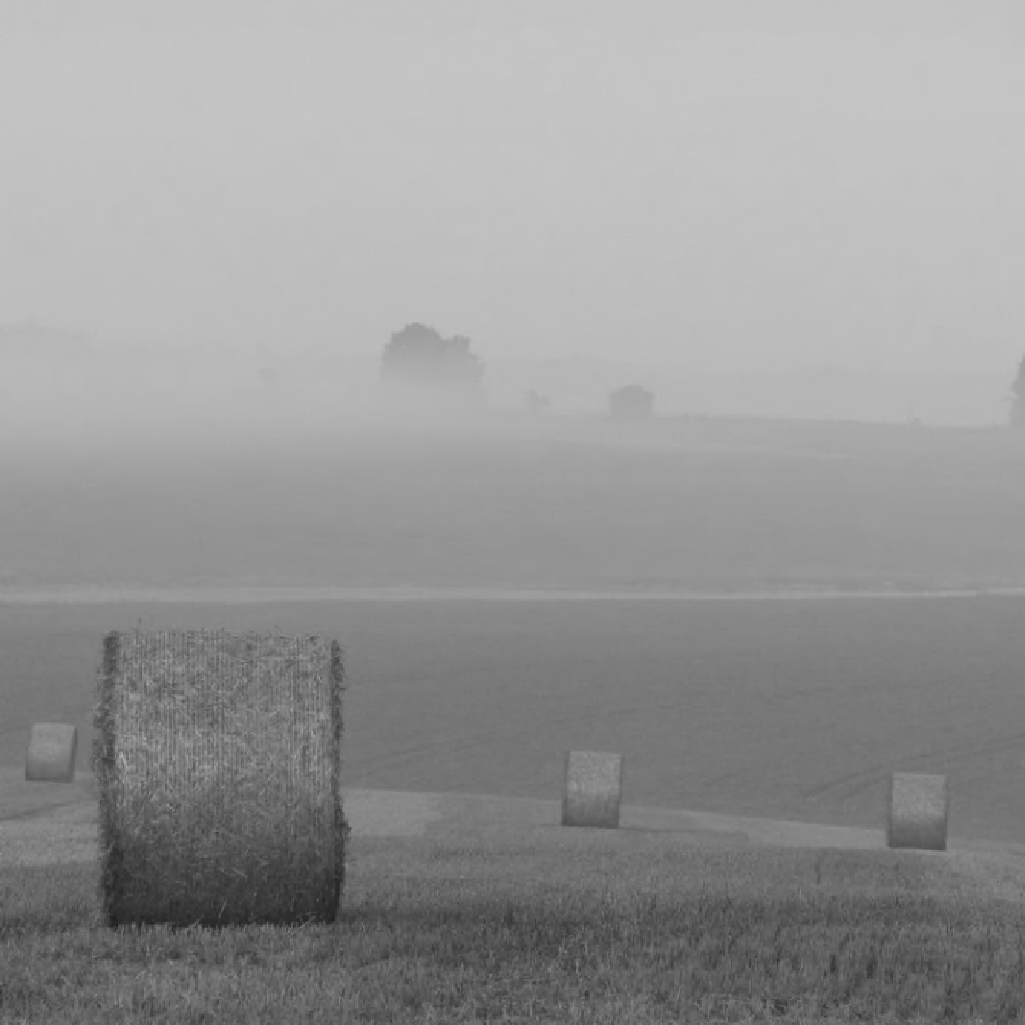
\includegraphics[width=0.4\textwidth]{./RawPictures/stogi-szare.png} }}%
    \qquad
    \subfloat{{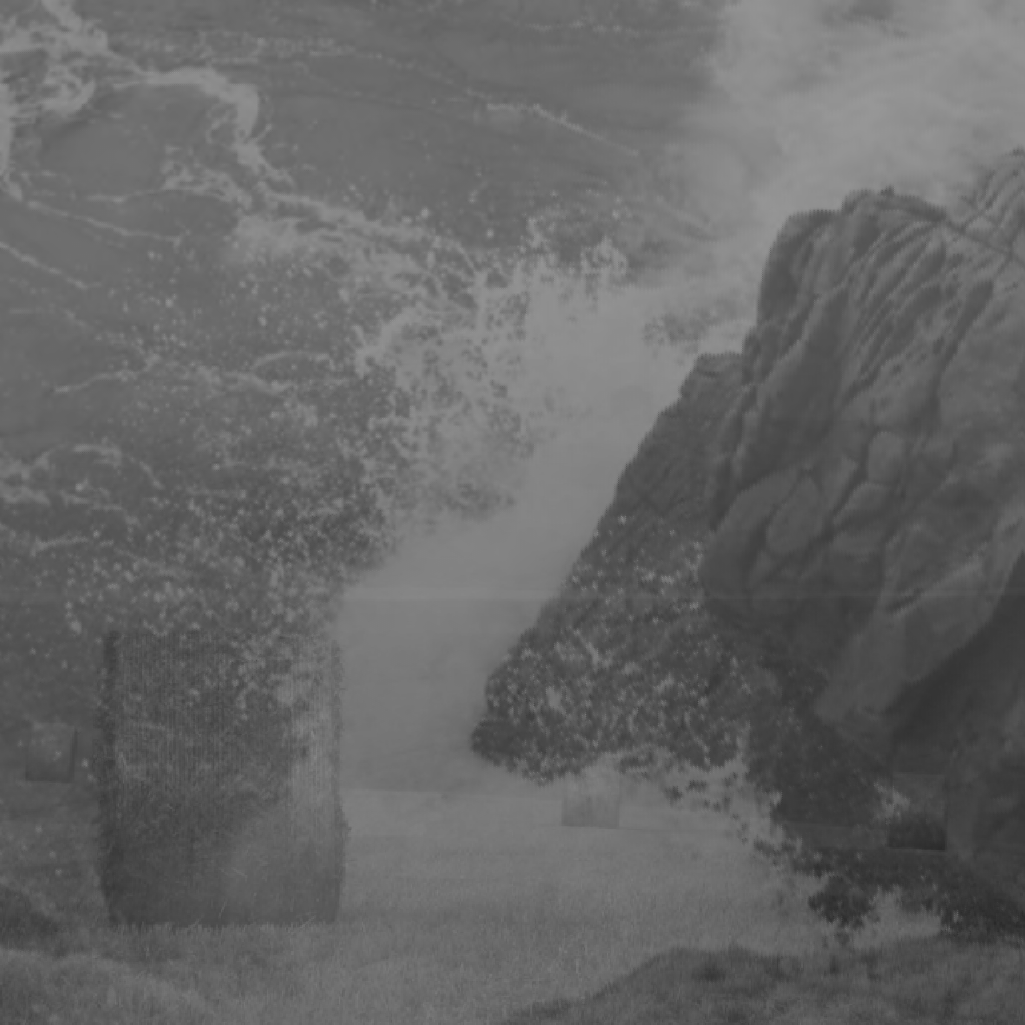
\includegraphics[width=0.4\textwidth]{./ExEffects/2/21/morze-szare_added_stogi-szare.png} }}%
    \subfloat{{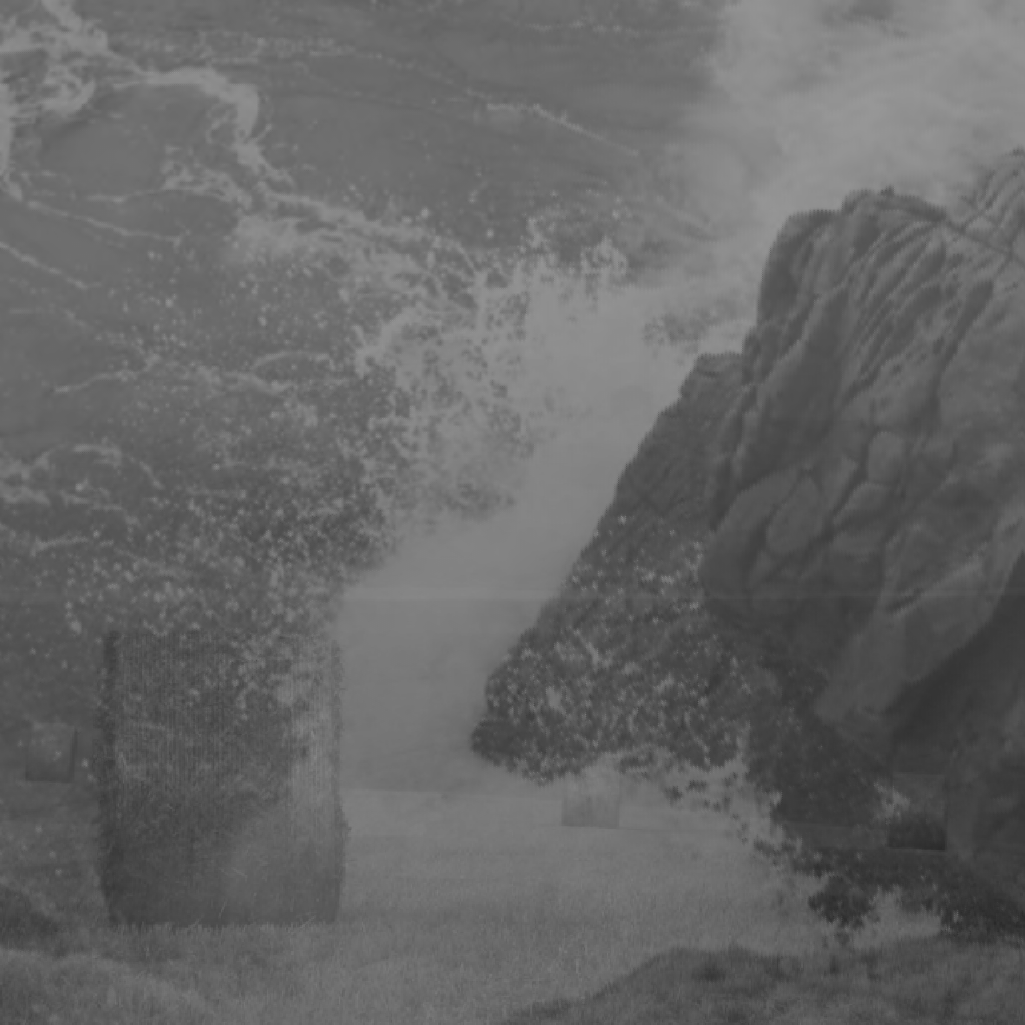
\includegraphics[width=0.4\textwidth]{./ExEffects/2/21/morze-szare_added_stogi-szare_normalized.png} }}%
    \caption{[Od lewej, rząd 1] Szary obraz wejściowy 1, szary obraz wejściowy 2 [Od lewej, rząd 2] Obraz po sumowaniu obrazów 1 i 2, obraz po normalizacji}%
    \label{fig:geo_after_grey1}%
\end{figure}
\FloatBarrier
\subsection*{Kod źródłowy algorytmu}
\begin{lstlisting}[language=Python]
def addPictureGrey(self):
    if self.checkPictureBits(self.pic1) == self.checkPictureBits(self.pic2):
        maxBitsColor = self.checkPictureBits(self.pic2)
    # check if pictures have same sizes, if not unify them
    compare = Comparer()
    biggerPicture, smallerPicture = compare.comparePictures(self.pic1, self.pic2)
    if biggerPicture != 0 and smallerPicture != 0:
        self.pic1, self.pic2 = self.getUnifiedPictures()
    # get the values
    tempName = smallerPicture.getPictureName()
    length1, width1, pictureName1 = self.pic1.getPictureParameters()
    matrix1 = self.pic1.getGreyMatrix()
    length2, width2, pictureName2 = self.pic2.getPictureParameters()
    matrix2 = self.pic2.getGreyMatrix()
    pictureName1 = tempName

    sumMax = 0
    x = 0
    fmax = 0
    fmin = maxBitsColor

    result = np.zeros((length1, width1), np.uint8)

    for l in range(length1):
        for w in range(width1):
            added = int(matrix1[l, w]) + int(matrix2[l, w])
            if sumMax < added:
                sumMax = added

    if sumMax > maxBitsColor:
        x = (sumMax - maxBitsColor) / maxBitsColor

    for l in range(length1):
        for w in range(width1):
            # Rounded up and assignment of value to the result matrix
            pom = int(matrix1[l, w] - (matrix1[l, w] * x)) + int(matrix2[l, w] - (matrix2[l, w] * x))
            result[l, w] = np.ceil(int(pom))
            # Search for maximum and minimum
            if fmin > pom:
                fmin = pom
            if fmax < pom:
                fmax = pom

    # save picture with added constant to png file (without normalization)
    path = self.ex + str(pictureName1) + '_added_' + str(pictureName2) + '.png'
    self.saver.savePictureFromArray(result, self.pictureType, path)

    normalized = np.zeros((length1, width1), np.uint8)
    for l in range(length1):
        for w in range(width1):
            normalized[l, w] = maxBitsColor*((result[l, w] - fmin) / (fmax - fmin))

    # save picture with added constant to png file (with normalization)
    path = self.ex + str(pictureName1) + '_added_' + str(pictureName2) + '_normalized.png'
    self.saver.savePictureFromArray(result, self.pictureType, path)
\end{lstlisting}

\section{Mnożenie obrazów szarych przez określoną stałą}
\subsection*{Opis algorytmu}
\par Algorytm mnożenia obrazu szarego przez określoną stałą polega na przemnożeniu każdego elementu obrazu (piksla) przez określoną stałą (skalar). Dla wszystkich piksli w obrazie wykonaj:
\begin{enumerate}
\item Jeżeli wartość piksla jest równa 255 to składowa wynikowa otrzymuje wartość stałej.
\item Jeżeli wartość piksla jest równa 0 to składowa wynikowa otrzymuje wartość 0.
\item Jeżeli wartość piksla jest inna niż 255 lub 0 to składowa wynikowa otrzymuje wartość poprzez pomnożenie wartości piksla przez skalar, podzielenie przez 255 i zaokrąglenie do liczby całkowitej.
\end{enumerate}
\subsection*{Efekty wykorzystania algorytmu}
\begin{figure}[h]
    \centering
    \subfloat{{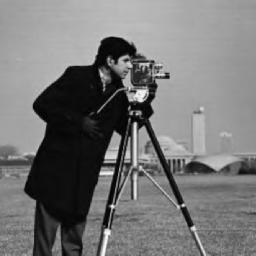
\includegraphics[width=0.3\textwidth]{./RawPictures/fotograf.png} }}%
    \subfloat{{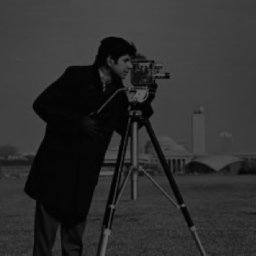
\includegraphics[width=0.3\textwidth]{./ExEffects/2/22/fotograf_constant_100.png} }}%
    \subfloat{{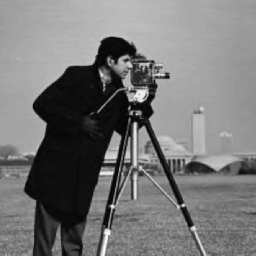
\includegraphics[width=0.3\textwidth]{./ExEffects/2/22/fotograf_constant_100_normalized.png} }}%
    \caption{[Od lewej] Szary obraz wejściowy, obraz po sumowaniu ze stałą 100, obraz po normalizacji}%
    \label{fig:geo_after_grey1}%
\end{figure}
\FloatBarrier
\begin{figure}[h]
    \centering
    \subfloat{{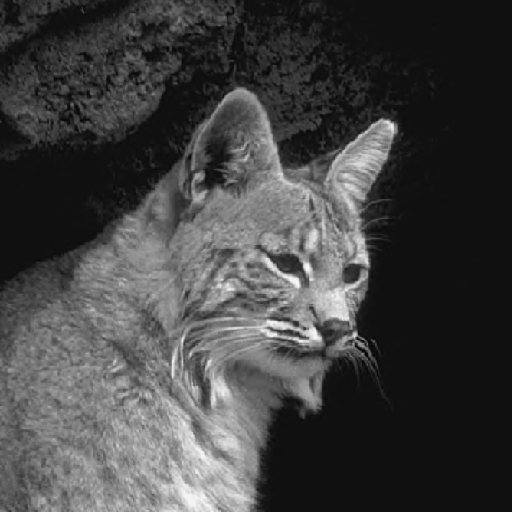
\includegraphics[width=0.3\textwidth]{./RawPictures/rys.png} }}%
    \subfloat{{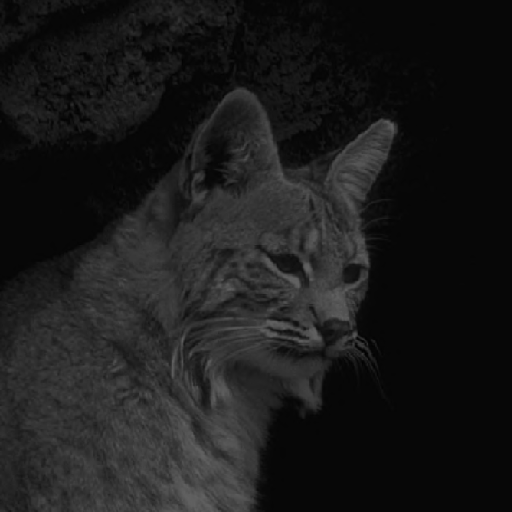
\includegraphics[width=0.3\textwidth]{./ExEffects/2/22/rys_constant_100.png} }}%
    \subfloat{{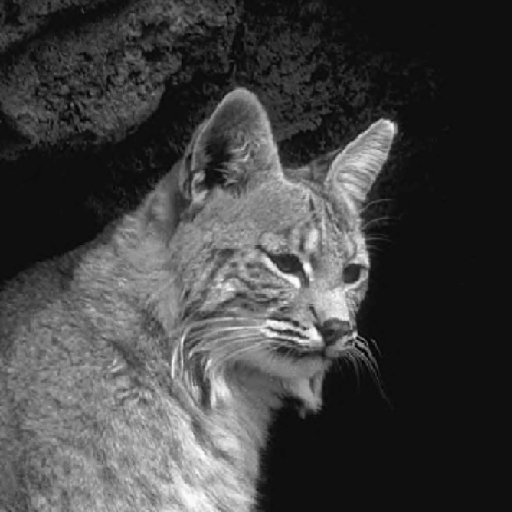
\includegraphics[width=0.3\textwidth]{./ExEffects/2/22/rys_constant_100_normalized.png} }}%
    \caption{[Od lewej] Szary obraz wejściowy, obraz po sumowaniu ze stałą 100, obraz po normalizacji}%
    \label{fig:geo_after_grey1}%
\end{figure}
\FloatBarrier
\subsection*{Kod źródłowy algorytmu}
\begin{lstlisting}[language=Python]
def multiplyConstGrey(self, constant):
    maxBitsColor = self.checkPictureBits(self.pic1)
    length, width, matrix, pictureName = self.getPictureParameters(self.pic1)
    result = np.ones((length, width), np.uint8)
    fmin = maxBitsColor
    fmax = 0
    for l in range(length):
        for w in range(width):
            pom = matrix[l, w]
            if pom == maxBitsColor:
                result[l, w] = maxBitsColor
            elif pom == 0:
                result[l, w] = 0
            else:
                result[l, w] = np.ceil(((matrix[l, w] * constant) / maxBitsColor))
            # Search for maximum and minimum
            if fmin > result[l, w]:
                fmin = result[l, w]
            if fmax < result[l, w]:
                fmax = result[l, w]
    # save picture with added constant to png file (without normalization)
    path = self.ex + str(pictureName) + '_constant_' + str(constant) + '.png'
    self.saver.savePictureFromArray(result, self.pictureType, path)
    for l in range(length):
        for w in range(width):
            result[l, w] = maxBitsColor*((result[l, w] - fmin) / (fmax - fmin))
    # save picture with added constant to png file (with normalization)
    path = self.ex + str(pictureName) + '_constant_' + str(constant) + '_normalized.png'
    self.saver.savePictureFromArray(result, self.pictureType, path)
\end{lstlisting}

\section{Mnożenie obrazu przez inny obraz}
\subsection*{Opis algorytmu}
\par Algorytm mnożenia obrazu szarego przez drugi szary obraz o tych samych wymiarach \(MxN\) i strukturze ich macierzy polega na przemnożeniu wartości piksla z pierwszego obrazu przez wartość odpowiadającego piksla z drugiego obrazu. Po operacji mnożenia następuje normalizacja obrazu. Dla każdego piksla pierwszego obrazu wykonaj następujące czynności:
\begin{enumerate}
\item Jeżeli wartość piksla \(P1[l,w]\) jest równa 255 to składowa wynikowa otrzymuje wartość odpowiadającego piksla drugiego obrazu \(P2[l,w]\).
\item Jeżeli wartość piksla \(P1[l,w]\) jest równa 0 to składowa wynikowa otrzymuje wartość 0.
\item Jeżeli wartość piksla \(P1[l,w]\) jest inna niż 255 lub 0 to składowa wynikowa otrzymuje wartość poprzez pomnożenie wartości piksla \(P1[l,w]\) przez odpowiadający piksel \(P2[l,w]\), podzielenie przez 255 i zaokrąglenie do liczby całkowitej.
\end{enumerate}
\subsection*{Efekty wykorzystania algorytmu}
\begin{figure}[h]
    \centering
    \subfloat{{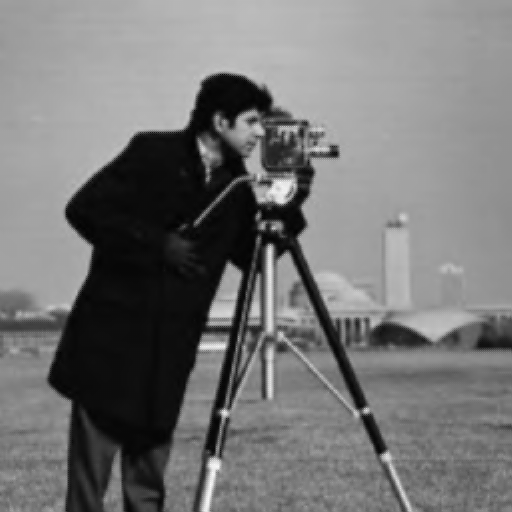
\includegraphics[width=0.4\textwidth]{./ExEffects/1/12/fotograf_rys_withInterpolation.png} }}%
    \subfloat{{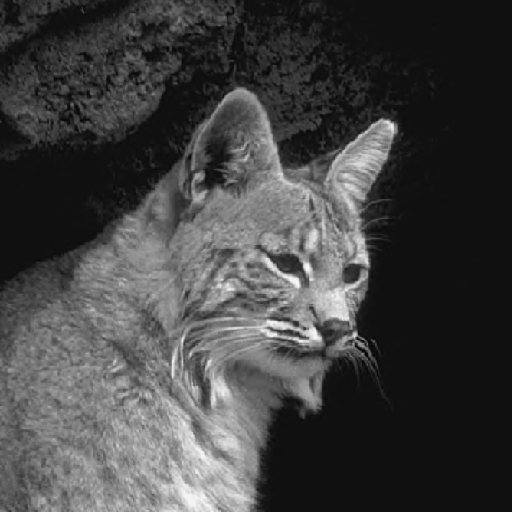
\includegraphics[width=0.4\textwidth]{./RawPictures/rys.png} }}%
    \qquad
    \subfloat{{\includegraphics[width=0.4\textwidth]{./ExEffects/2/22/fotograf_multiplied_rys.png} }}%
    \subfloat{{\includegraphics[width=0.4\textwidth]{./ExEffects/2/22/fotograf_multiplied_rys_normalized.png} }}%
    \caption{[Od lewej, rząd 1] Szary obraz wejściowy 1, szary obraz wejściowy 2 [Od lewej, rząd 2] Obraz po sumowaniu obrazów 1 i 2, obraz po normalizacji}%
    \label{fig:geo_after_grey1}%
\end{figure}
\FloatBarrier
\begin{figure}[h]
    \centering
    \subfloat{{\includegraphics[width=0.4\textwidth]{./ExEffects/1/12/fotograf_AndrzejZamoyski_withInterpolation.png} }}%
    \subfloat{{\includegraphics[width=0.4\textwidth]{./RawPictures/AndrzejZamoyski.png} }}%
    \qquad
    \subfloat{{\includegraphics[width=0.4\textwidth]{./ExEffects/2/22/fotograf_multiplied_AndrzejZamoyski.png} }}%
    \subfloat{{\includegraphics[width=0.4\textwidth]{./ExEffects/2/22/fotograf_multiplied_AndrzejZamoyski_normalized.png} }}%
    \caption{[Od lewej, rząd 1] Szary obraz wejściowy 1, szary obraz wejściowy 2 [Od lewej, rząd 2] Obraz po sumowaniu obrazów 1 i 2, obraz po normalizacji}%
    \label{fig:geo_after_grey1}%
\end{figure}
\FloatBarrier
\subsection*{Kod źródłowy algorytmu}
\begin{lstlisting}[language=Python]
def multiplyPicturesGrey(self):
    if self.checkPictureBits(self.pic1) == self.checkPictureBits(self.pic2):
        maxBitsColor = self.checkPictureBits(self.pic2)
    # check if pictures have same sizes, if not unify them
    compare = Comparer()
    biggerPicture, smallerPicture = compare.comparePictures(self.pic1, self.pic2)
    if biggerPicture != 0 and smallerPicture != 0:
        self.pic1, self.pic2 = self.getUnifiedPictures()
    # get the values
    tempName = smallerPicture.getPictureName()
    length1, width1, matrix1, pictureName1 = self.getPictureParameters(self.pic1)
    length2, width2, matrix2, pictureName2 = self.getPictureParameters(self.pic2)
    pictureName1 = tempName

    result = np.ones((length1, width1), np.uint8)

    fmin = maxBitsColor
    fmax = 0

    for l in range(length1):
        for w in range(width1):
            if matrix1[l, w] == maxBitsColor:
                result[l, w] = matrix2[l, w]
            elif matrix1[l, w] == 0:
                result[l, w] = 0
            else:
                result[l, w] = np.ceil(((int(matrix1[l, w]) * int(matrix2[l, w])) / maxBitsColor))
            # Search for maximum and minimum
            if fmin > result[l, w]:
                fmin = result[l, w]

            if fmax < result[l, w]:
                fmax = result[l, w]

    # save picture multiplied by picture to png file (without normalization)
    path = self.ex + str(pictureName1) + '_multiplied_' + str(pictureName2) + '.png'
    self.saver.savePictureFromArray(result, self.pictureType, path)

    for l in range(length1):
        for w in range(width1):
            result[l, w] = maxBitsColor*((result[l, w] - fmin) / (fmax - fmin))

    # save picture multiplied by picture to png file (with normalization)
    path = self.ex + str(pictureName1) + '_multiplied_' + str(pictureName2) + '_normalized.png'
    self.saver.savePictureFromArray(result, self.pictureType, path)
\end{lstlisting}

\section{Mieszanie obrazów z określonym współczynnikiem}

\section{Potęgowanie obrazu z zadaną potęgą}
\section{Dzielenie obrazów szarych przez zadaną stałą}
\section{Dzielenie obrazu przez inny obraz}
\section{Pierwiastkowanie obrazu}
\section{Logarytmowanie obrazu}

\chapter{Operacje sumowania arytmetycznego obrazów barwowych}

\section{Sumowanie obrazów barwowych}
\subsection{Sumowanie obrazu z określoną stałą}
\subsection{Sumowanie dwóch obrazów}
\section{Mnożenie obrazów barwowych}
\subsection{Mnożenie obrazu przez określoną stałą}
\subsection{Mnożenieobrazu przez inny obraz}
\section{Mieszanie obrazów z określonym współczynnikiem}
\section{Potęgowanie obrazu z zadaną potęgą}
\section{Dzielenie obrazów barwowych}
\subsection{Dzielenie obrazu przez zadaną stałą}
\subsection{Dzielenie obrazu przez inny obraz}
\section{Pierwiastkowanie obrazu}
\section{Logarytmowanie obrazu}

\chapter{Operacje geometryczne na obrazie}
\section{Przemieszczanie obrazu o zadany wektor}
\section{Skalowanie obrazu}
\subsection{Skalowanie jednorodne}
\subsection{Skalowanie niejednorodne}
\section{Obracanie obrazu o dowolny kąt}
\section{Symetrie obrazu}
\subsection{Symetra względem osi OX}
\subsection{Symetria względem osi OY}
\subsection{Symetria względem zadanej prostej}
\section{Wycinanie fragmentów obrazów}
\section{Kopiowanie fragmentów obrazów}

\chapter{Operacje na histogramie obrazu szarego}
\section{Obliczanie histogramu}
\section{Przemieszczanie histogramu}
\section{Rozciąganie histogramu}
\section{Progowanie lokalne}
\section{Progowanie globalne}

\chapter{Operacje na histogramie obrazu barwowego}
\section{Obliczanie histogramu}
\section{Przemieszczanie histogramu}
\section{Rozciąganie histogramu}
\section{Progowanie 1 progowe lokalne}
\section{Progowanie 1 progowe globalne}
\section{Progowanie wieloprogowe lokalne}
\section{Progowanie wieloprogowe globalne}

\end{document}
